\documentclass[a4paper,11pt,uplatex]{ujreport}
\usepackage{style/nislab,style/thesis}
\usepackage{tabularx}

%----------------------------------------------------------------------
% 修論・卒論 執筆 注意事項
%----------------------------------------------------------------------
% 章立て
% * 章のなかに節が1つだけの場合は,節を立てる必要がありません.節の中に小節が1つだけの場合も同様です.
% * つまり,chapterの中には,sectionは2つ以上あるべきで,sectionが1つの場合は,そのsectionは不要で,chapter直下に内容を記述すべきです.
% * 論文の概要と「はじめに」(イントロダクション)は異なるものです.概要は結果も含めた論文全体の概要であり,「はじめに」は解決すべき問題を明示するための背景情報および論文でその問題をどう取り扱うかの導入について記載するものです.

% 背景と目的
%   * 最初に「背景と目的」を書くのが一般的かと思いますが,「背景と目的」は論文の概要ではありません.
%   * なぜ,この研究をする必要があるのか,一般的な世間の状況と,研究を行う必要性を書くことになります.
%   * 単に今までに無かったので作ったではダメです(例:AとBをつなぐシステムが無かったので作りました)
%   * 世の中でその問題にどう取り組んでいるかは,一般には「関連研究」のところで説明します.
%   * 一般的な背景情報はこの章にまとめてください(本文中に一般的背景情報を書くべきではありません)
%   * また,この章では,論文の技術的な内容や結果を書く必要がありません.なぜなら「背景と目的」だからです.
%   * 一方,論文の「概要」は,研究結果および論文の結論まで含めて書くべきです.

% 提案方式の説明
%   * 問題に関して,自分の解決方法を説明します.
%   * 問題そのものを簡単に理解できない場合は,問題についても詳解が必要です.
%   * 問題をどうやって解決するかを手順を追って解説します.
%   * 複数の問題が関連している場合は問題を分離して説明します.
%   * 自分の解決方法が従来とどこが違いどう工夫しているかを明記する必要があります.

% 評価
%   * 自分の解決方法を問題点に適応してどういう結果が得られたかについて説明をします.
%   * 従来技術や手法と比較してどこがどうよくなったかを示します.
%   * どのような環境で比較したかを説明する必要があります.
%   * 定量的に以前(関連研究)と比べてこうよくなったと説明できればベターです.

% 考察
%   * なるべくなら考察を章で分けて下さい.提案方式に関する「評価」に関して記載する章があるのが一般的かと思いますが,「考察」の章では,従来技術や関連研究と比較して,評価結果がどうであったかを考察して下さい.

% まとめ (★特に修論の場合の注意点★)
%   * 800 字から1000字ぐらいでまとめてください.
%   * 背景,解決すべき問題点,提案内容,結果,考察,研究の意義などを含めて記載してください.
%   * 結果については,過去形(・・・実施した.・・・評価した.・・・確認した.など)で記載してください.

% 参考文献
%   * 勉強した書籍を列挙するものではありません.
%   * 本文中に引用した技術などを記載するものです.
%   * 参考文献の番号は,必ず本文中の引用場所を示します.(本文中に引用の番号がない参考文献は存在しません)

% 表現
%   * 自分が出した結果に対して「・・・と考えられる」や「・・・と言える」は使わないで下さい.
%   * 関連研究などの他人の出した結論に対しては OK.
%   * 一般的に断言できない場合は,条件を設定して「・・・という条件においては,・・・である」と断定してください.
%   * 文中に副詞を用いる場合は,その副詞が本当に必要かどうかをよく考えて下さい.
%   * 略語は,論文の最初に登場したところで何の略語であるかを記載して下さい.
%   * 文中は定量的な表現を使って下さい.大きい/小さい,長い/短い,速い/遅い,など.何をもって大きいと言えるのか,などを考えて下さい.

% ページ数
%   * 修論は本文が20ページ以内.図を含めて20ページを越えても問題ありません.
%   * 卒論は20ページ以上で記載して下さい.
%   * 出版物になりますので,権利関係が明確になっていない場合,同志社大学あるいはその関係者以外に著作権のある図の利用は不可です.

% 提出
%   * 必ず,締切の前日までに事務に提出してください.締切の当日に(交通機関の遅延,病気などの一般的には正当な理由があっても)遅れた場合は受理されません.

%----------------------------------------------------------------------
% 表紙用
%----------------------------------------------------------------------
\type{1}  % 1:卒業論文 2:修士論文
\title{ホームネットワークにおけるデータ特性を考慮したSDNによる優先度制御手法}  % 日本語タイトル
\etitle{SDN Based Priority Control Method Considering Data Attributes for Home Network}  % 英語タイトル
\author{国本 典晟}  % 著者
\date{2022年2月10日}  % 日付
\advisor{佐藤 健哉 教授}  % 指導教員
\university{同志社大学} % 大学名
\department{理工学部 情報システムデザイン学科} % 専攻
\lab{ネットワーク情報システム研究室}  % 研究室
\entryyear{2018}  % 入学年度
\studentnumber{1033}  % 学生番号

%----------------------------------------------------------------------
% 変更不要
%----------------------------------------------------------------------
\begin{document}
\maketitle
\clearpage

%----------------------------------------------------------------------
% 概要
%----------------------------------------------------------------------
% 卒業論文は日本語(200~400文字),修士論文は英語(200~300単語)で書く.
% 改行は不要
%----------------------------------------------------------------------
\begin{abstract}
  %   * 概要は,論文全体を読まなくてもその研究の序論から結論までが理解できるようにするものです.本文の内容を忠実に反映させるだけでなく,研究の新規性や重要性を簡潔かつ的確に伝えられることが,より多くの読者を獲得する鍵となります.概要は,研究目的から研究方法,研究結果,そして結論に至る肝心な要素のすべてが要約されていなければならないのです.

  SDNのホームネットワークへの適用が期待されているが,ホームネットワークには特性の異なるデータの通信が混在し,通信の種類と量が時間帯によって変動するため,それらの制御方法が課題となっている.現在のインターネットサービスプロバイダはデータ特性を考慮せず制御を行うため,通信帯域の逼迫の際に重要なパケットの損失などの問題が生じる.また,従来の優先度分類では,テレワークの増加などの昨今のリアルタイム性の高い通信の需要を十分に考慮できておらず,優先度が固定されていたため状況に応じた優先度制御が困難であった.本研究では,リアルタイム性を含むデータ特性から通信を4つに分類し,動的に優先度を設定し,優先度制御を行う手法を提案した.ホームネットワークを想定したネットワークを構築して実験を行い,先行研究と比較してリアルタイム性の点で改善し,状況に応じて優先すべき通信の性能が向上した.

\end{abstract}

% キーワードを3つ設定する
% 卒業論文は日本語,修士論文は英語
\addkeywords{SDN}{ホームネットワーク}{分類アルゴリズム}

%----------------------------------------------------------------------
% 変更不要
%----------------------------------------------------------------------
\footnote[0]{本論文に掲載の製品名・会社名等は,一般にそれぞれの会社の商標,または登録商標である.}
\footnote[0]{なお,本文中では\texttrademark ・ \textregistered 等のマークは特に明記していない.}

%----------------------------------------------------------------------
% 変更不要
%----------------------------------------------------------------------
% ページ番号をギリシャ数字にする
\pagenumbering{roman}

% 目次を1ページから始めるために表紙を0ページにする
\setcounter{page}{0}

% 目次を作成
\tableofcontents

% 改ページ
\clearpage

% 以降,ページ番号をアラビア数字で振り直す
\pagenumbering{arabic}

%----------------------------------------------------------------------
% はじめに
%----------------------------------------------------------------------
\chapter{はじめに}
\label{chap:Introduction}

%   * 最初はイントロ的なことを書く.\par

\section{背景}
\label{sec:背景}

%   * 最近の現状と問題点とか.\par

  Software-Defined Networking(SDN)とは,\figref{fig:sdn}のようにネットワーク制御機能とデータ転送機能を分離し,データ転送機能のみをネットワーク機器に担わせ,外部のソフトウェアが一括してネットワークの制御を行う技術の総称である.
  SDN登場以前,ルータなどのネットワーク機器はネットワークを制御する機能とデータを転送する機能を併せ持っていたため,ネットワークにおける制約が大きく,環境の変化に対応するのが困難であった.
  SDNにより,ネットワークをソフトウェアで集中制御することで,ネットワークの仮想化,迅速・柔軟な変更,管理の効率化などが可能になり,企業ネットワークやInformation and Communication Tecknology(ICT)システムなどに利用されている\cite{NEC}.\par
  一方,ホームネットワークの拡張や複雑化のため,SDNのホームネットワークへの適用が期待されている.
  ホームネットワークとは,PCやスマートフォン,Internet of Things(IoT)機器などから構成されるLAN環境を家庭内に構築したものである.
  近年,画像や動画データなどの大容量データの需要の拡大やIoT機器の普及に伴い,ホームネットワークとインターネット間の通信量が急速に増加し,通信帯域の逼迫が危惧されている\cite{ガイドライン}.
  現在,ホームネットワークとインターネット間の通信を管理しているインターネットサービスプロバイダ(ISP)は,通信の重要度やQuality of Service(QoS)要件といった特性を考慮せず制御しているが,通信帯域が逼迫した際に重要なパケットの損失やQoSの低下などの問題が生じる恐れがある.
  この問題の解決のため,SDNを利用してISPがホームネットワークを集約して最適化された帯域制御を行う方式が提案されている\cite{Framework}.\par
  ホームネットワークには,重要度やQoS要件などのデータ特性の異なる通信が混在している.
  例えば,緊急事態を通知するデータは重要度が高いため遅延やパケットの損失が許されず,動画データは多少のパケットの損失は許されるが大きく遅延してはならない.
  また,近年ではテレワークの増加に伴い,切断されるとリアルタイム性が損なわれるデータの需要が高まっている.
  加えて,ホームネットワークはユーザや時間帯による通信の種類と量の変動が大きく,ユーザや家庭の状況によって通信の重要度や需要も変化する.
  こうした重要度やQoS要件,リアルタイム性などのデータ特性が異なる通信を状況に応じて制御するには,データ特性から通信を分類して動的に優先度を設定し,SDNを用いて通信帯域に応じてパケットの破棄などを行う優先度制御が必要である.

  \begin{figure}[!tb]
    \centering
    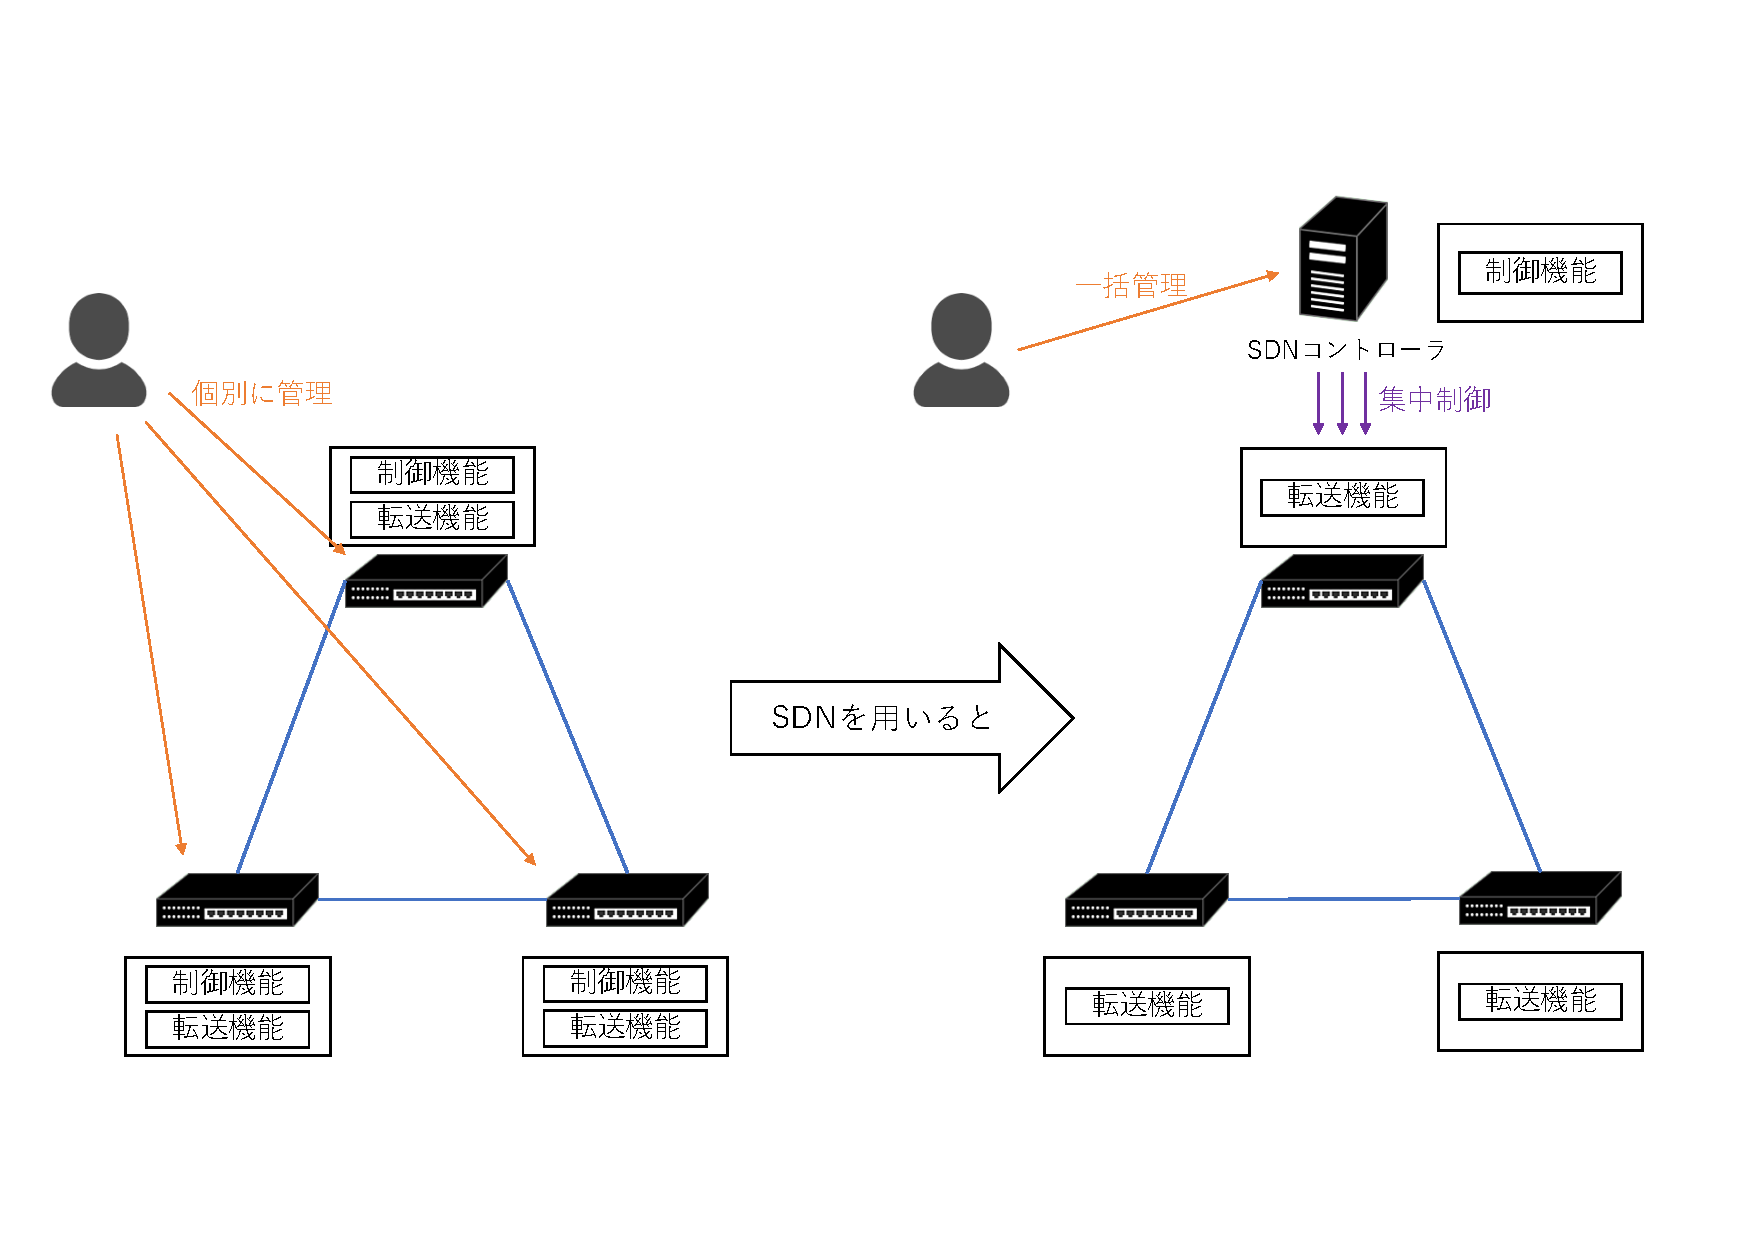
\includegraphics[width=\linewidth]{img/SDN_trimmed.pdf}
    \caption{SDNの概要}
    \label{fig:sdn}
  \end{figure}

\section{目的}
\label{sec:目的}

    本研究では,ホームネットワークの制御において問題となるデータ特性が異なる通信や通信の種類と量の変動を解決するため,データ特性を考慮して通信を分類し,動的な優先度制御を行う手法を提案し,状況に応じた優先度の高い通信の品質を改善する.
    また,リアルタイム性を考慮し,優先度制御に伴うパケットの破棄による通信への影響を軽減することを目的とする.
    ホームネットワークを想定したネットワークを構築して実験を行い,提案手法の有効性を評価する.

%アインシュタイン方程式は以下の通りである.\par

%\begin{equation}
%  R_{\mu\nu} - \frac{1}{2} g_{\mu\nu} R = \frac{8\pi G}{c^2} T_{\mu\nu}
%\end{equation}

%ベクトルの書き方は以下の通り.\par

%\begin{itemize}
%  \item 普通の$\alpha$は\verb|\alpha|で書く。
%  \item \verb|$\vec{\alpha}$| で $\vec{\alpha}$
%  \item \verb|\usepackage{bm}| している場合は
%        \verb|$\bm{\alpha}$| で $\bm{\alpha}$
%  \item 並べると,$\alpha$, $\vec{\alpha}$, $\bm{\alpha}$
%\end{itemize}

\section{本論文の構成}
\label{sec:本論文の構成}

  第\ref{chap:関連研究}章では,SDNをホームネットワークに適用するために,通信の遅延要件や帯域保証を基準に優先度分類を行なった関連研究について述べる.第\ref{chap:提案手法}章では,第\ref{chap:関連研究}章で注目されたデータの特性に合わせて,さらにリアルタイム性を考慮した通信の分類と,動的に優先度を設定し通信帯域に応じて優先度の低い通信のパケットを破棄するアドミッション制御について述べる.第\ref{chap:評価}章では,提案手法の有効性の評価のための実験方法とその評価結果について述べる.第\ref{chap:考察}章では,実験によって得られた結果に対して考察を行う.第\ref{chap:おわりに}章では,本論文のまとめを述べる.

%----------------------------------------------------------------------

\chapter{関連研究}
\label{chap:関連研究}

\section{遅延要件による優先度分類}
\label{sec:遅延要件による優先度分類}

  Jangらは,3GPP Long Term Evolutionが定義したQoS Class Identifier(QCI)をホームネットワークの通信に適用できるよう,\tabref{tab:QCI}のように再定義した\cite{Framework}.
  さらに,各QCIの遅延要件(\tabref{tab:QCI}のPacket Delay Budget)を基準にして通信を3つのカテゴリに分類し,各カテゴリに割り当てる通信帯域の割合を動的に変更することで,QoSとQoE(Quality of Experience)の改善を目指した\cite{Framework2}.\par
  しかし,通信帯域を割り当てるのみで,優先度の高い通信のために優先度の低い通信のパケットを破棄する優先度制御を行わないため,QCI=5に示されるミッションクリティカルな通信のパケットが損失してしまう恐れがある.
  また,QCI=3の通信とQCI=4の通信を同様に制御するなど,通信のリアルタイム性を考慮しておらず,通信帯域が逼迫した際に通信品質への影響が懸念される.

  %\begin{figure}[!b]
    %\centering
    %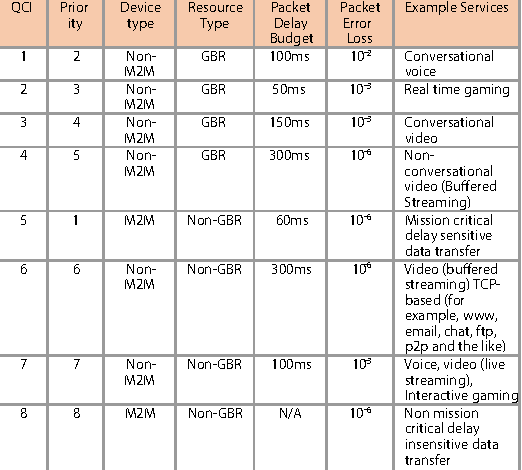
\includegraphics[]{img/qci.pdf}
    %\caption{ホームネットワーク用に再定義されたQCI}
    %\label{fig:qci}
  %\end{figure}

  \newcolumntype{A}{>{\centering\arraybackslash}p{3mm}}
  \newcolumntype{B}{>{\centering\arraybackslash}p{7mm}}
  \newcolumntype{C}{>{\centering\arraybackslash}p{8mm}}
  \begin{table}[!b]
    \caption{スマートホームサービス向けに再定義されたQCI}
    \label{tab:QCI}
    \centering
    {\scriptsize
    \begin{tabularx}{\linewidth}{ABBCCBX}
      \hline
      QCI & Priority & Device type & Resource Type & Packet Delay Budget & Packet Error Loss & \multicolumn{1}{c}{Example Services}\\
      \hline \hline
      1 & 2 & Non-M2M & GBR & 100ms & $10^{-2}$ & Conversational voice\\
      2 & 3 & Non-M2M & GBR & 50ms & $10^{-3}$ & Real time gaming\\
      3 & 4 & Non-M2M & GBR & 150ms & $10^{-3}$ & Conversational video\\
      4 & 5 & Non-M2M & GBR & 300ms & $10^{-6}$ & Non-conversational video (Buffered streaming)\\
      5 & 1 & M2M & Non-GBR & 60ms & $10^{-6}$ & Mission critical delay sensitive data transfer\\
      6 & 6 & Non-M2M & Non-GBR & 300ms & $10^{-6}$ & Video (Buffered streaming) TCP-based (for example,www,email,chat,ftp,p2p and the like)\\
      7 & 7 & Non-M2M & Non-GBR & 100ms & $10^{-3}$ & Voice,Video (Live streaming),Interactive gaming\\
      8 & 8 & M2M & Non-GBR & N/A & $10^{-6}$ & Non mission critical delay insensitive data transfer\\
      \hline
    \end{tabularx}
    }
  \end{table}

\section{帯域保証による優先度分類}
\label{sec:帯域保証による優先度分類}

  Dengらは,JangらのQCIを基に,帯域保証(\tabref{tab:QCI}のResource Type)を基準として優先度を分類した\cite{AQRA}.
  また,最も優先度の高い通信のQoS要件を満たすため,優先度の低い通信のパケットを破棄するアドミッション制御を行なった.
  これにより,ミッションクリティカルな通信のQoS要件を満たした.\par
  しかし,\ref{sec:遅延要件による優先度分類}節と同様に,QCI=3とQCI=4の通信を同じ優先度で制御しており,通信のリアルタイム性を考慮できていない.
  また,優先度分類の基準を帯域保証のみとしたため,遅延要件とパケットロス要件の厳しいQCI=7の通信が最も優先度が低く分類されてしまっている.
  さらに,固定された優先度分類を元にアドミッション制御を行うため,優先度分類と実際の通信の重要度や需要が異なる状況においても,固定された優先度分類において優先度が低い通信のパケットを破棄してしまう.

%----------------------------------------------------------------------
\chapter{提案手法}
\label{chap:提案手法}

  本研究では,第\ref{chap:関連研究}章で述べた,ミッションクリティカルな通信のパケットが損失する恐れがある問題や,通信のリアルタイム性を考慮していない問題,固定された優先度分類と通信の重要度や需要が異なる状況に対応できない問題を解決するために,リアルタイム性を含むデータ特性を考慮した通信の分類と,動的に優先度を設定し優先度の高い通信の品質を改善するアドミッション制御を提案する.本章では,まずSDNによるホームネットワークとISP間のネットワーク管理について述べ,その後通信の分類とアドミッション制御について述べる.

\section{SDNによるネットワーク管理}
\label{sec:SDNによるネットワーク管理}

  ホームネットワークにはPCやスマートフォン,IoT機器など様々な通信機器が存在しているが,それらは\figref{fig:homenetwork}のように,有線または無線で全て家庭用ルータに接続されており,家庭用ルータを介してインターネットに接続している.
  本論文では,このような家庭用ルータを「ゲートウェイ」と表記する.

  \begin{figure}[!b]
    \centering
    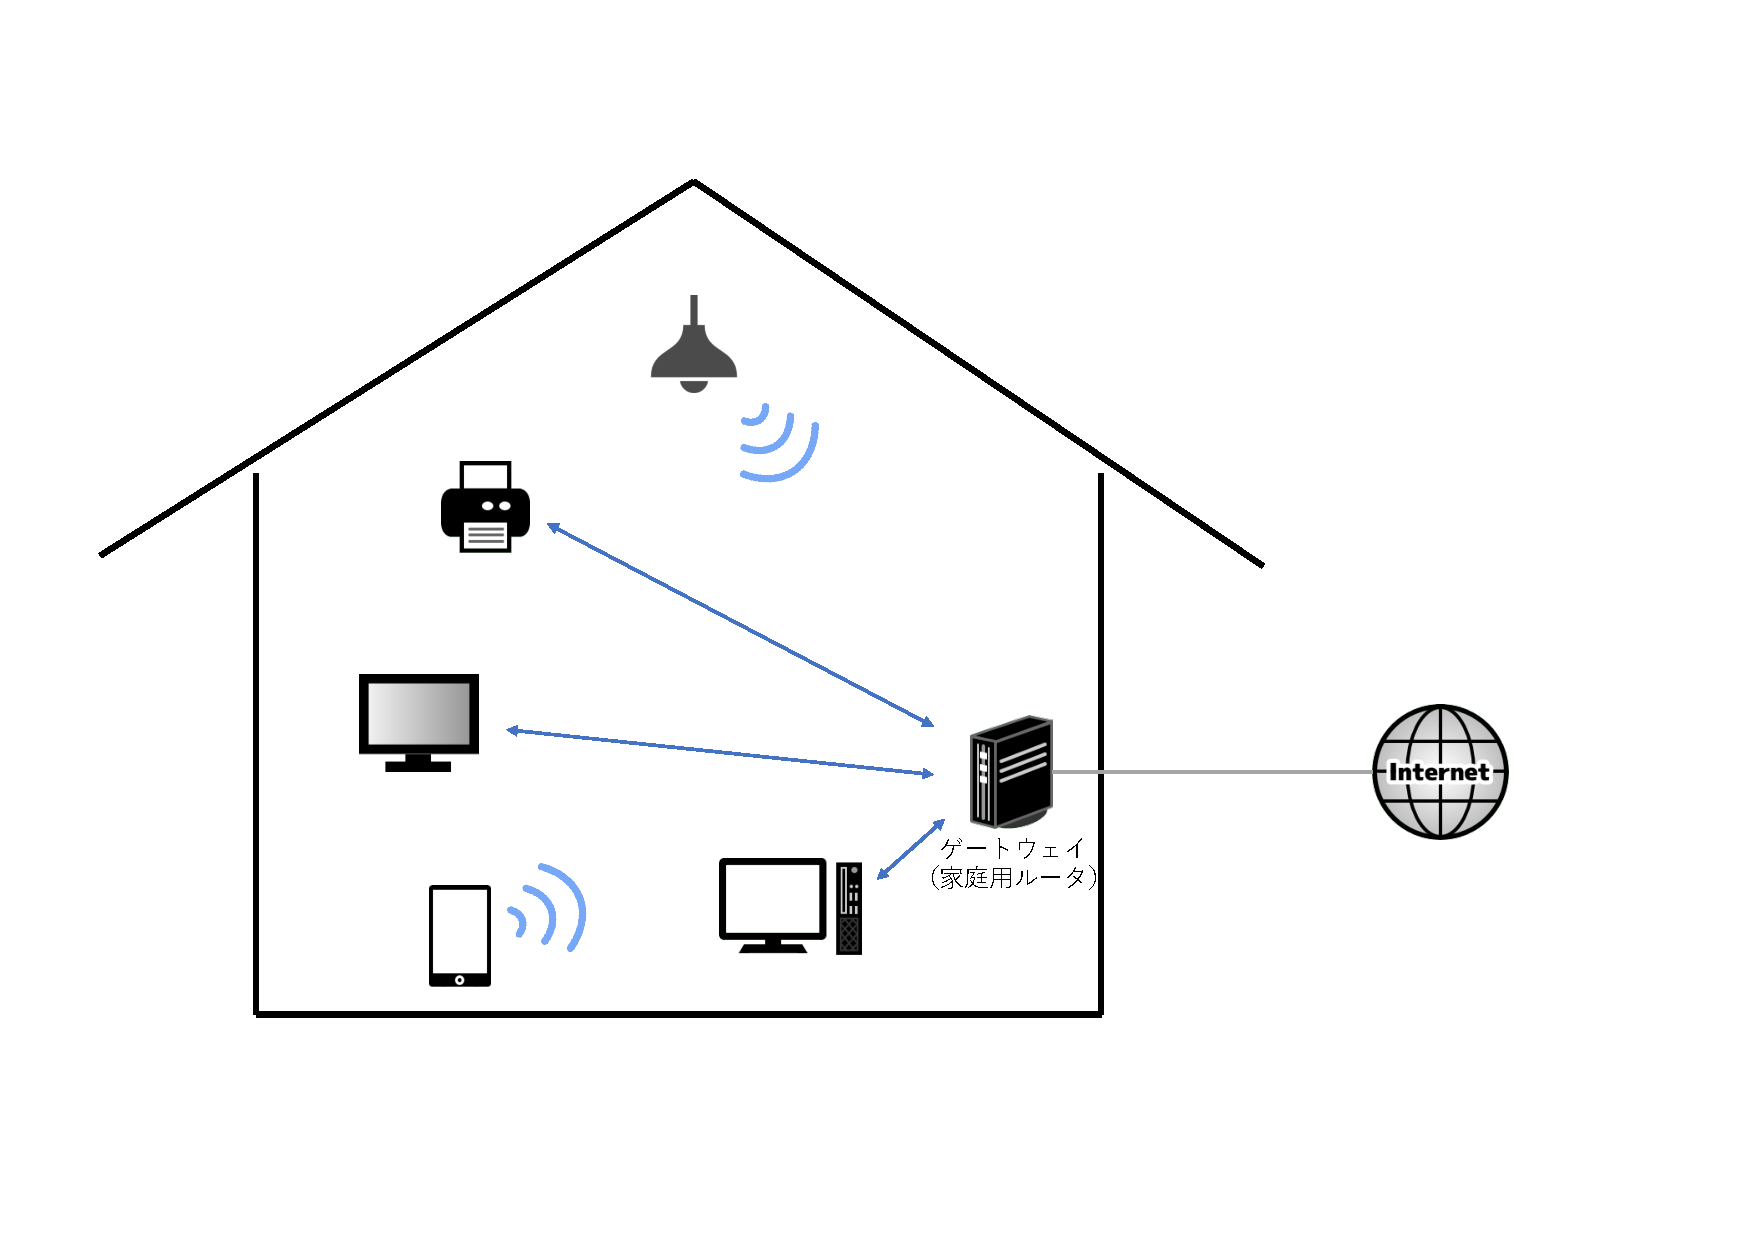
\includegraphics[width=\linewidth]{img/homenetwork_trimmed.pdf}
    \caption{ホームネットワークの構造}
    \label{fig:homenetwork}
  \end{figure}

  ホームネットワークがインターネットに接続するには,\figref{fig:ISP}に示すように,アクセスネットワークとISPを経由する必要がある.
  ホームネットワーク内で発生したデータは,アクセスネットワークを経由し,ISPが管理するサーバへと到達する.
  ISPは,サーバにてホームネットワークで発生したデータをインターネットへ接続するための処理を行い,インターネットへデータを送信する.
  本論文では,アクセスネットワーク内のデータの中継機を「ルータ」,ISPが管理するサーバを「ISPサーバ」と総称する.\par

  \begin{figure}[!tb]
    \centering
    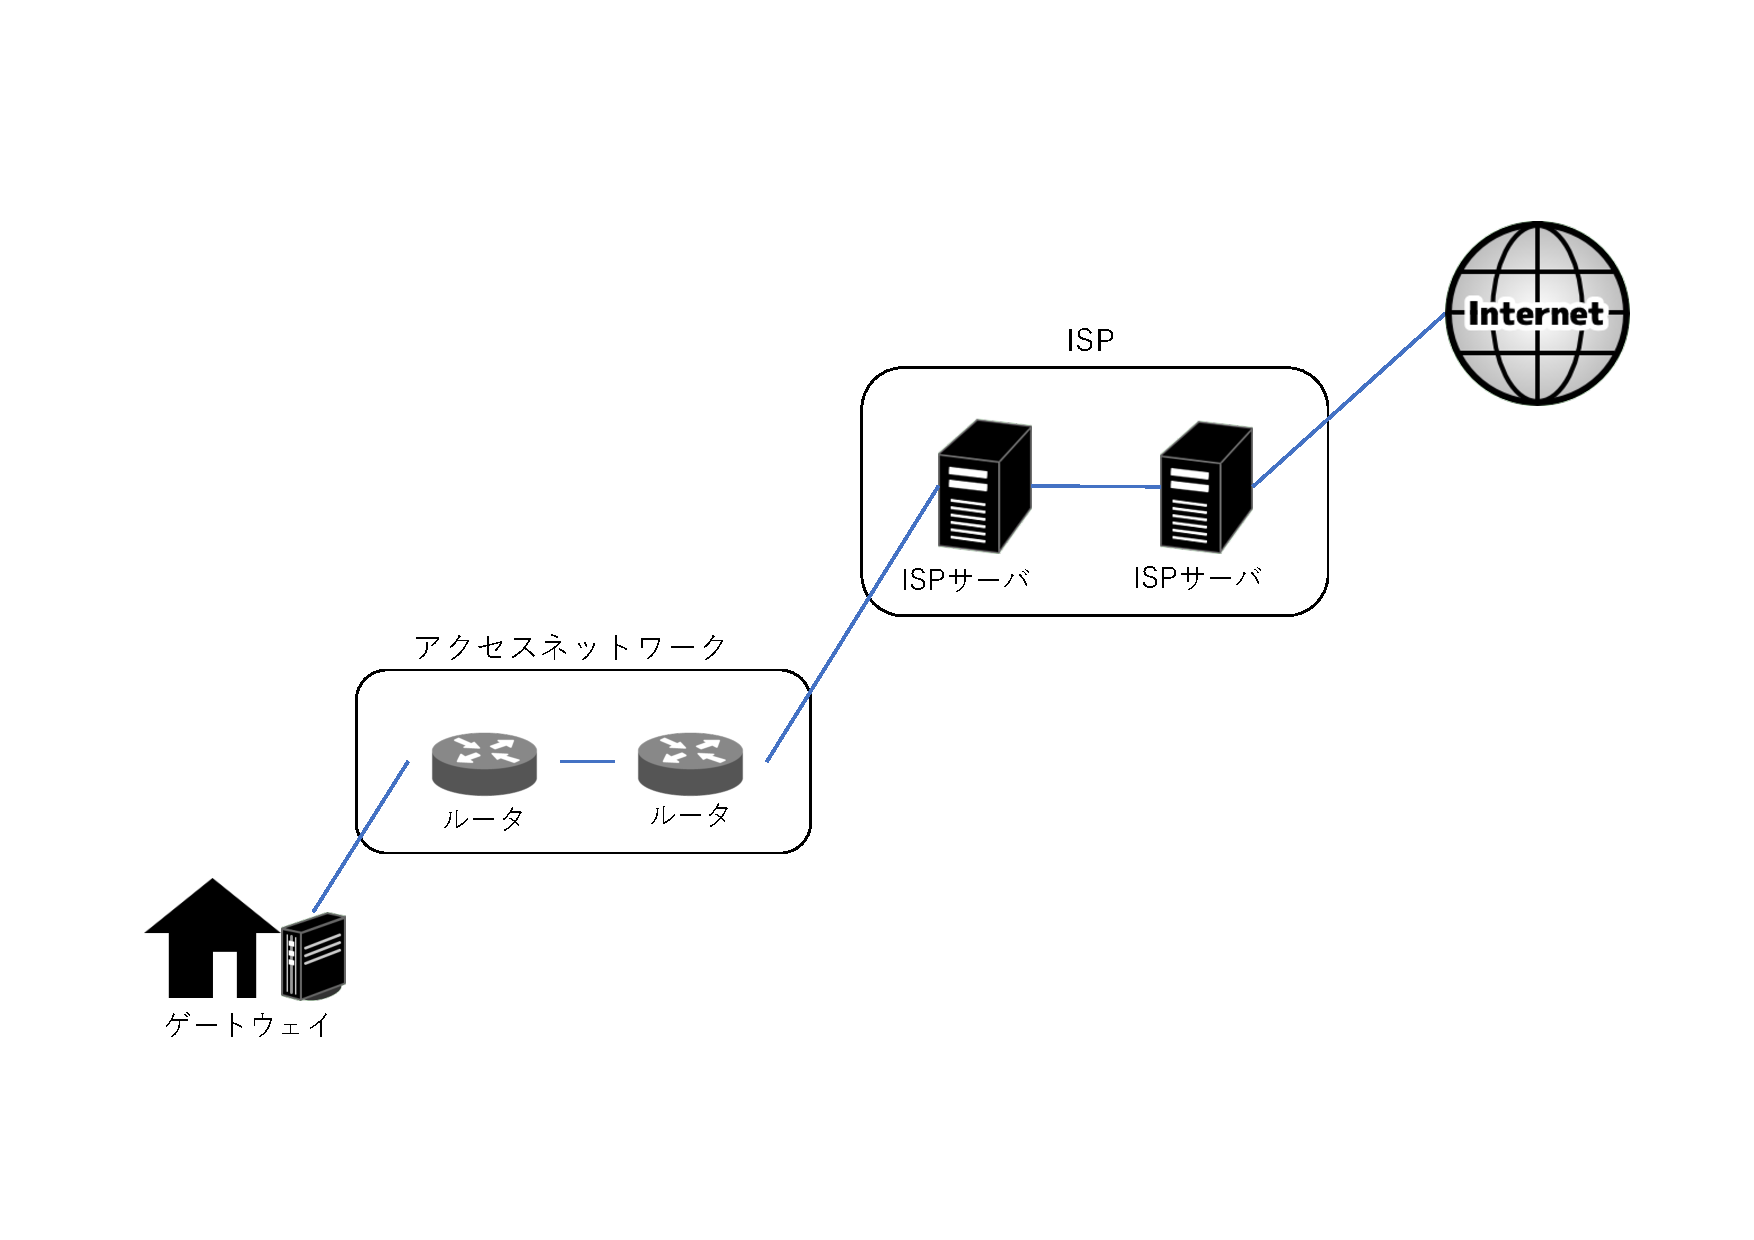
\includegraphics[width=\linewidth]{img/ISP_trimmed.pdf}
    \caption{ホームネットワークとインターネット間のネットワーク}
    \label{fig:ISP}
  \end{figure}

  \ref{sec:背景}節で述べた通り,SDNとはネットワーク制御機能とデータ転送機能を分離し,データ転送機能のみをネットワーク機器に担わせ,外部のソフトウェアが一括してネットワークの制御を行う技術の総称である.
  ホームネットワークとISP間のネットワークにSDNを適用するには,データ転送機能を担うネットワーク機器とネットワーク制御機能を担うソフトウェアが必要となる.
  データ転送機能を担うネットワーク機器は,\figref{fig:ISP}のゲートウェイ,ルータ,ISPサーバが該当する.
  ネットワーク制御機能を担うソフトウェアとして,新たにSDNコントローラを配置する.
  SDNによるネットワーク管理を\figref{fig:proposal}に示す.
  SDNコントローラはゲートウェイ,ルータ,ISPサーバと接続しており,これらとネットワーク制御に必要なメッセージをやりとりすることで,ネットワーク全体の制御を行う.
  また,SDNコントローラは,アクセスネットワークの通信帯域やホームネットワークの状況に応じて,\ref{sec:通信の分類}節で述べる通信の分類を,\ref{sec:アドミッション制御}節で述べるように優先度を設定しアドミッション制御をゲートウェイに指示する.
  ゲートウェイは,SDNコントローラの指示に従いアドミッション制御を行う.\par

  %\begin{figure}[!tb]
    %\centering
    %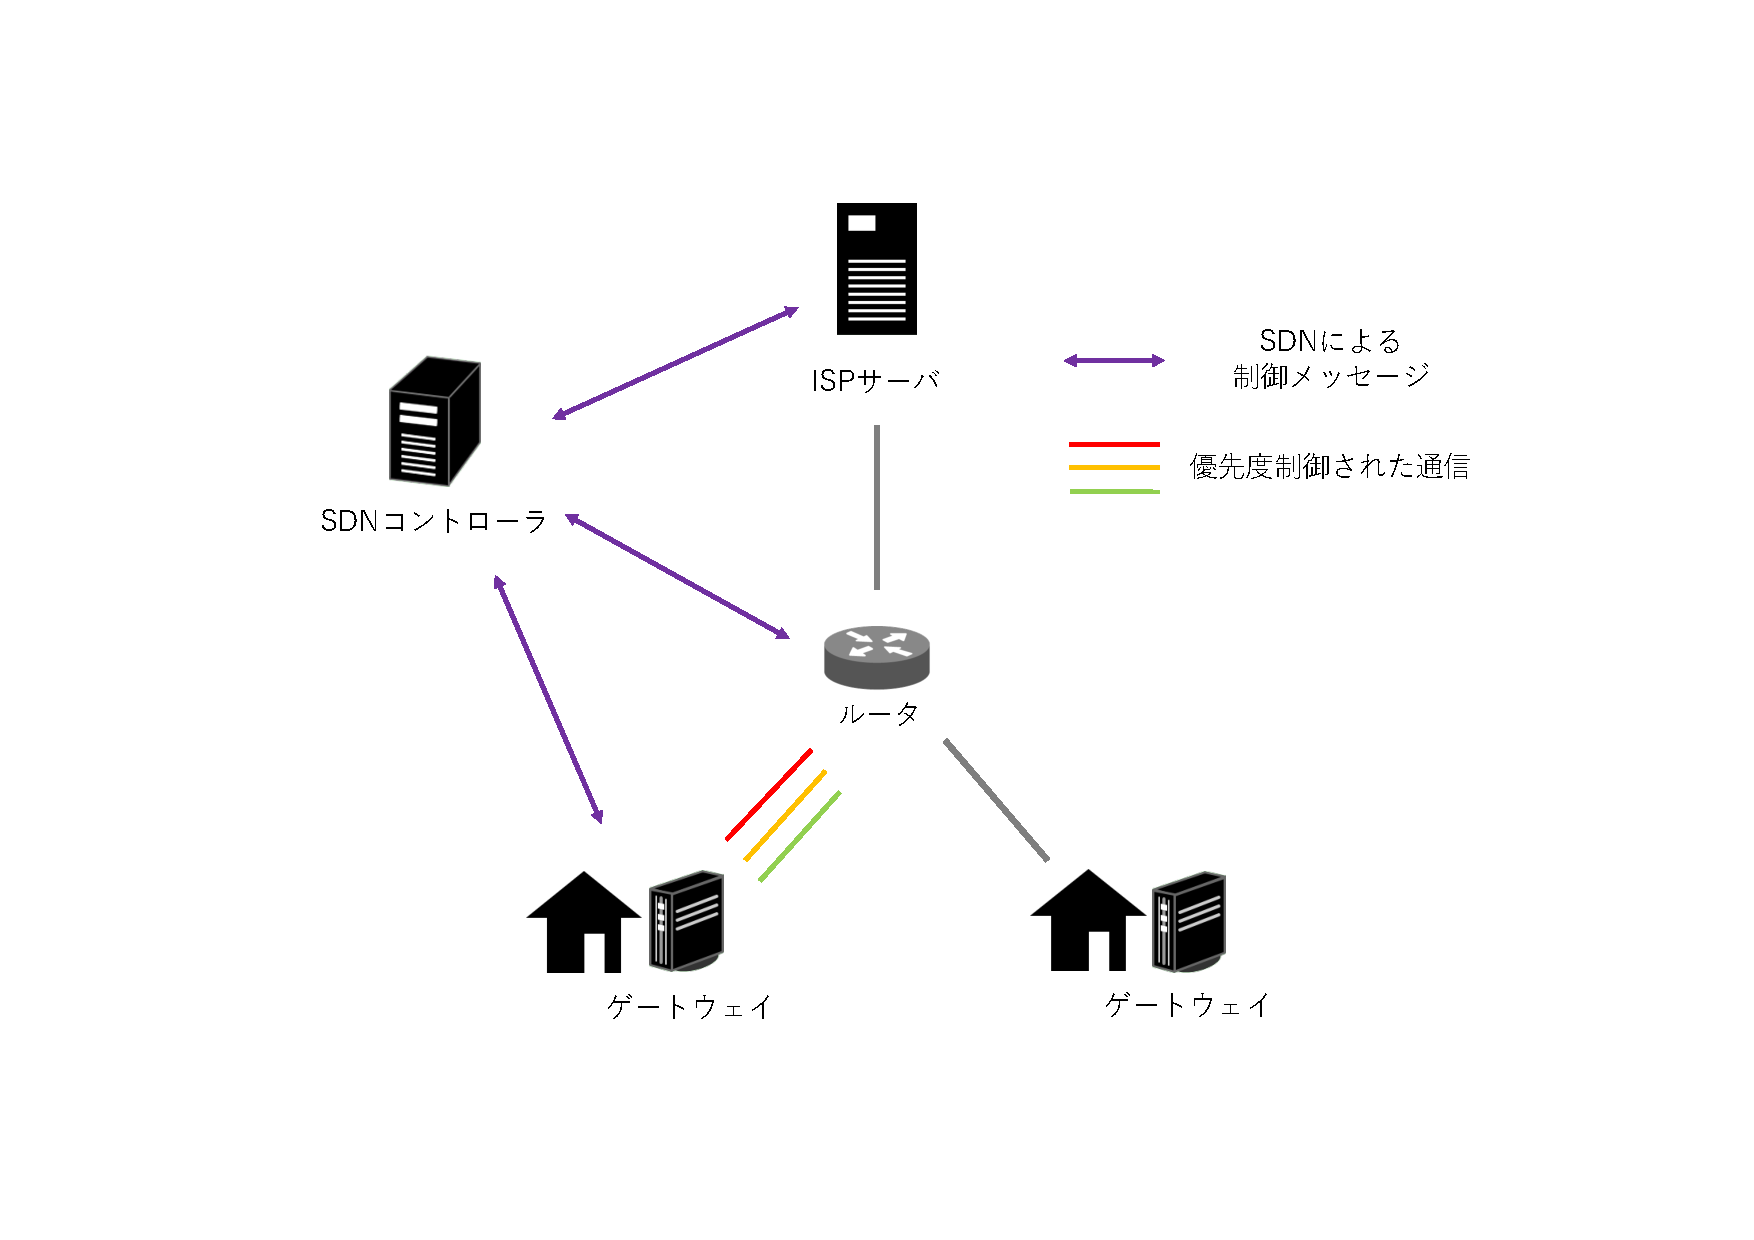
\includegraphics[width=\linewidth]{img/proposal.pdf}
    %\caption{SDNによるネットワーク管理}
    %\label{fig:proposal}
  %\end{figure}

\section{通信の分類}
\label{sec:通信の分類}

  ホームネットワークには重要度やQoS要件,リアルタイム性など,データ特性の異なる通信が混在している.
  SDNを用いてホームネットワークの通信を制御するために,以下のようにデータ特性を基準として通信を4種類のカテゴリに分類する.

  \clearpage

  \begin{figure}[!tb]
    \centering
    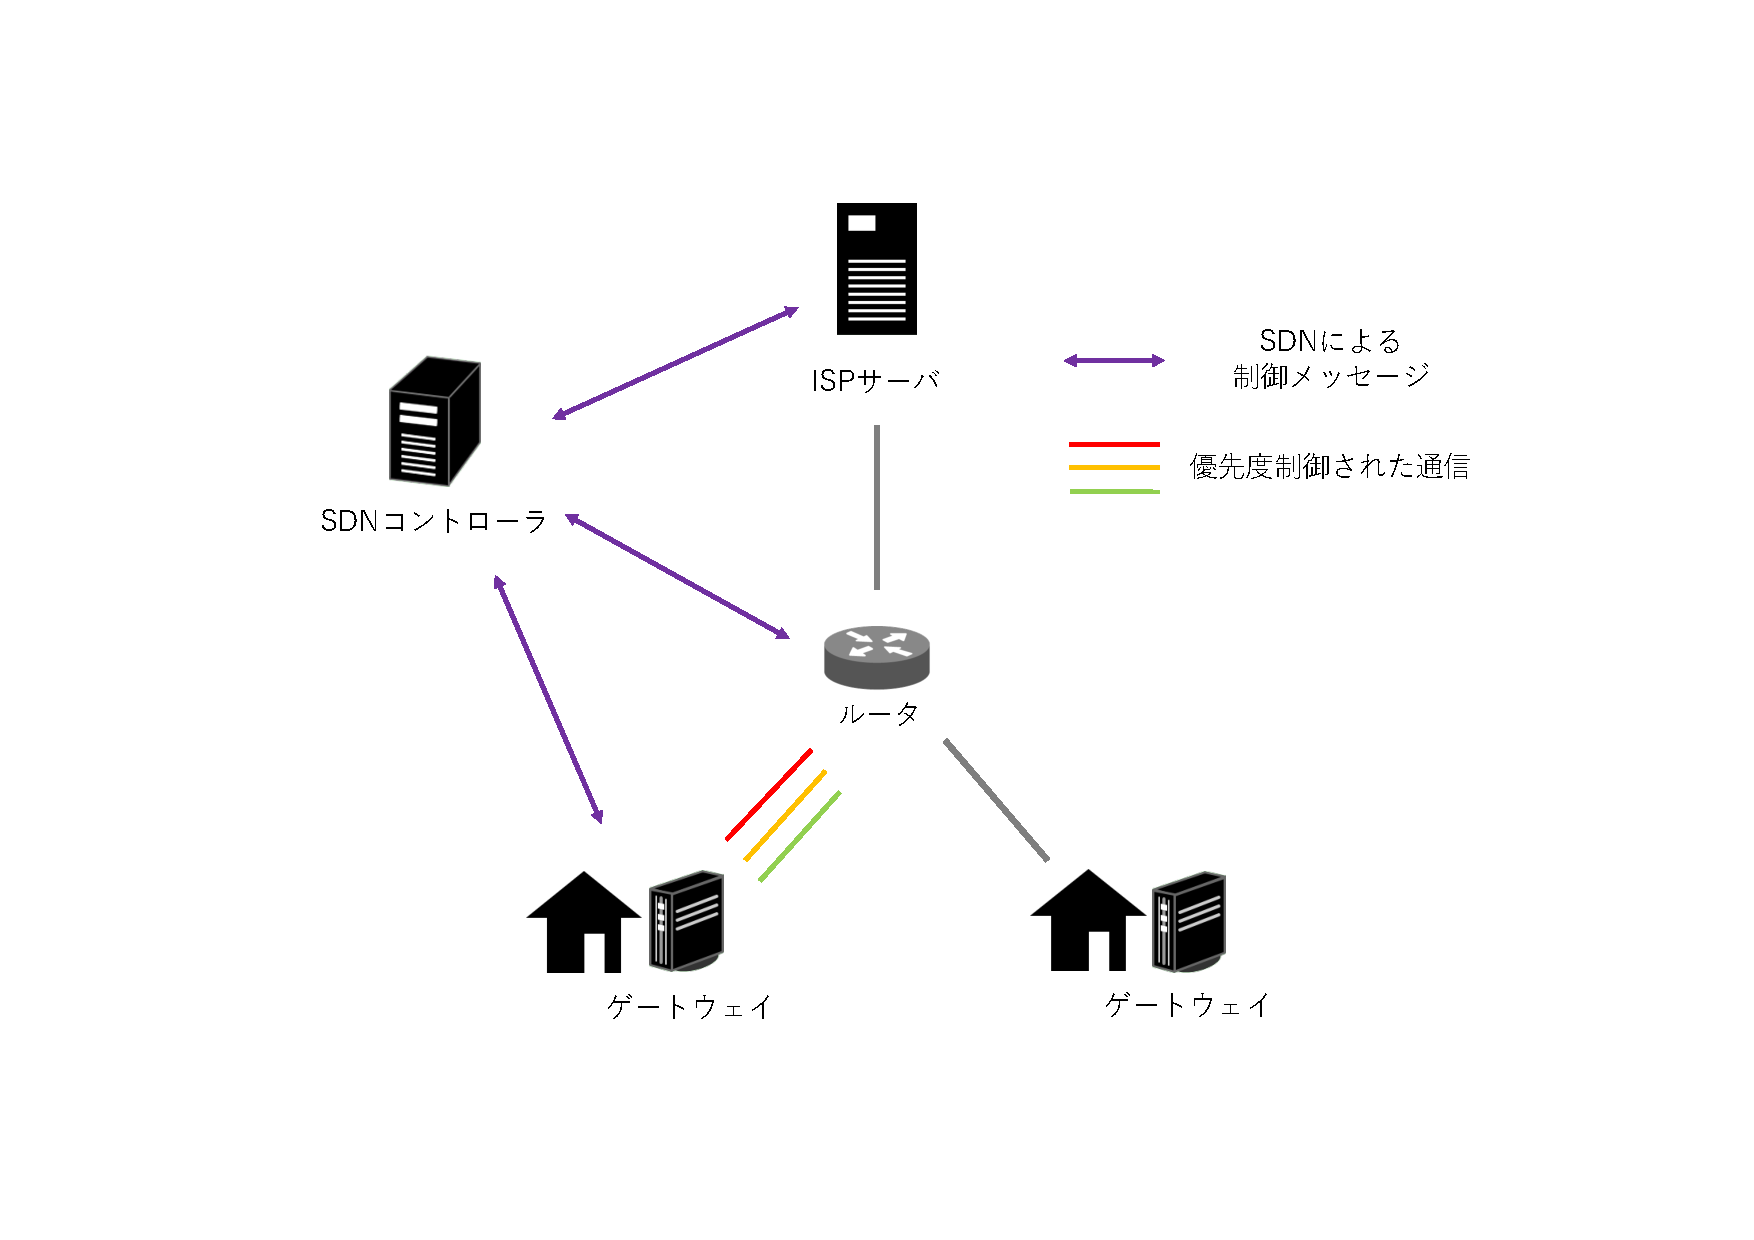
\includegraphics[width=\linewidth]{img/proposal.pdf}
    \caption{SDNによるネットワーク管理}
    \label{fig:proposal}
  \end{figure}

  \begin{itemize}
    \setlength{\leftskip}{1.0cm}
    \item[カテゴリ1]\mbox{}\\
          カテゴリ1には,火災報知器や侵入者センサなどのミッションクリティカルなデータの通信が該当する.
          ミッションクリティカルなデータは,遅延やパケットの損失が,生命の危機などの重大な事態につながる恐れがある.
          また,ミッションクリティカルなデータは通常データサイズが小さく,あまり通信帯域を消費しない.
          以上のことから,カテゴリ1は通常,最も高い優先度に設定される.
    \item[カテゴリ2]\mbox{}\\
          カテゴリ2には,音声通話やWeb会議などのリアルタイム性の高い音声・映像データの通信が該当する.
          音声・映像データは,遅延が大きい場合やパケットの損失が多い場合には,音声・映像が止まる,途切れるなどの恐れがある.
          また,音声通話やWeb会議などは人同士のコミュニケーションに用いられるためリアルタイム性が高く,これらの通信が途切れるとテレワークに支障をきたすなどの問題が発生する.
          以上のことから,カテゴリ2は通常,2番目に高い優先度に設定される.
    \item[カテゴリ3]\mbox{}\\
          カテゴリ3には,録画された動画などのリアルタイム性の低い音声・映像データの通信が該当する.
          カテゴリ3の音声・映像データの通信が途切れた場合,音声・映像の視聴が一時妨げられるなどの問題が発生するが,カテゴリ2と比較して通信品質への影響が小さい.
          以上のことから,カテゴリ3は通常,3番目に高い優先度に設定される.
    \item[カテゴリ4]\mbox{}\\   
          カテゴリ4には,WebサイトなどのTCPによる通信や室温センサなどの非ミッションクリティカルなデータの通信が該当する.
          これらの通信は遅延やパケットの損失の影響がカテゴリ1\textasciitilde3の通信と比較して小さく,通信が途切れても通信品質にあまり影響しない.
          以上のことから,カテゴリ4は通常,最も低い優先度に設定される.

  \end{itemize}

\section{アドミッション制御}
\label{sec:アドミッション制御}

  \ref{sec:通信の分類}節で述べた通り,カテゴリ1の通信のデータはミッションクリティカルであるため,遅延やパケットの損失が許されない.
  また,カテゴリ2の通信はリアルタイム性が高いため,遅延や切断の影響が大きい.
  ホームネットワークとISPサーバ間の通信帯域が逼迫した場合,カテゴリ1またはカテゴリ2の通信の遅延やパケットの損失の恐れがあるため,優先度の低い通信のフローを破棄することで,カテゴリ1またはカテゴリ2の通信のための通信帯域を確保するアドミッション制御を行う.\par

  SDNを実現する代表的な技術であるOpenFlowでは,宛先IPアドレスや宛先MACアドレス,宛先ポート番号などのルールが同じ通信の集合体を「フロー」と呼び,通信をフローごとに制御している.
  データ転送機能を担うネットワーク機器はフロー情報を内部に保存し,受信したパケットをフロー情報を参照して処理する.
  受信したパケットが保存しているフロー情報のいずれにも合致しない時,または必要に応じて,SDNコントローラはネットワーク機器に新たなフロー情報を送信し,ネットワーク機器はそのフロー情報に従い処理を行う.
  ここでは,SDNコントローラは,カテゴリ1またはカテゴリ2の通信に十分な通信帯域がない場合,優先度の低い通信のフローを破棄するようゲートウェイに指示することでアドミッション制御を行う.\par

  \begin{figure}[!tb]
    \centering
    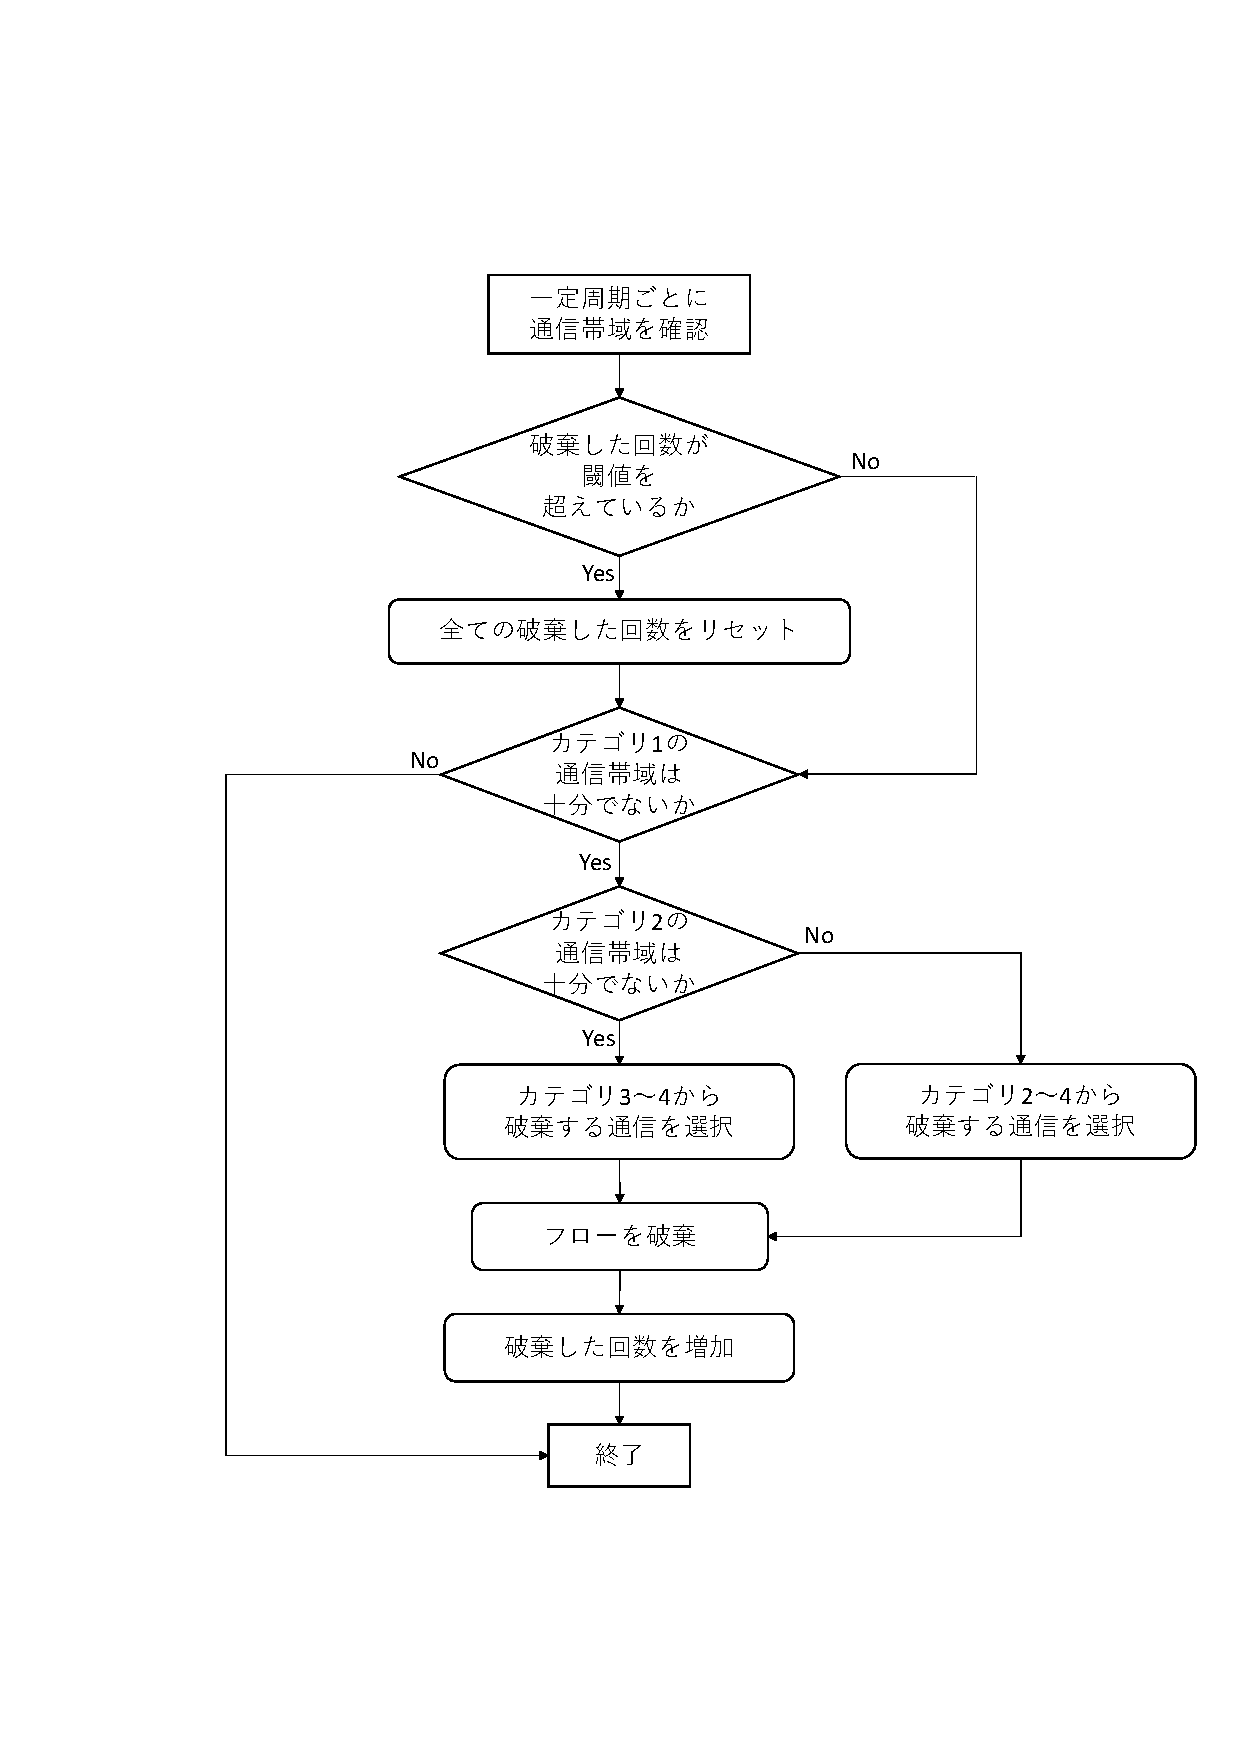
\includegraphics[width=\linewidth]{img/adomission_c1.pdf}
    \caption{カテゴリ1のためのアドミッション制御のフローチャート}
    \label{fig:adomission}
  \end{figure}

  カテゴリ1の通信のためのアドミッション制御のフローチャートを\figref{fig:adomission}に示す.
  SDNコントローラはゲートウェイとISPサーバ間の通信帯域を監視し,一定周期ごとにカテゴリ1またはカテゴリ2の通信に十分な通信帯域があるか確認する.
  カテゴリ1の通信に十分な通信帯域がなく,かつカテゴリ2の通信に十分な通信帯域がない場合,カテゴリ3またはカテゴリ4の通信のフローから破棄するフローを選択する.
  カテゴリ1の通信に十分な通信帯域がなく,カテゴリ2の通信に十分な通信帯域がある場合,カテゴリ2\textasciitilde4の通信のフローから破棄するフローを選択する.
  その後,SDNコントローラは選択したフローを破棄するようゲートウェイに指示し,ゲートウェイは指示に従いフローを破棄する.
  カテゴリ1の通信に十分な通信帯域がある場合でも,\figref{fig:adomission2}に示すフローチャートのように,カテゴリ2の通信に十分な通信帯域がない場合には,カテゴリ3\textasciitilde4の通信のフローを破棄するアドミッション制御を行う.\par

  \begin{figure}[!tb]
    \centering
    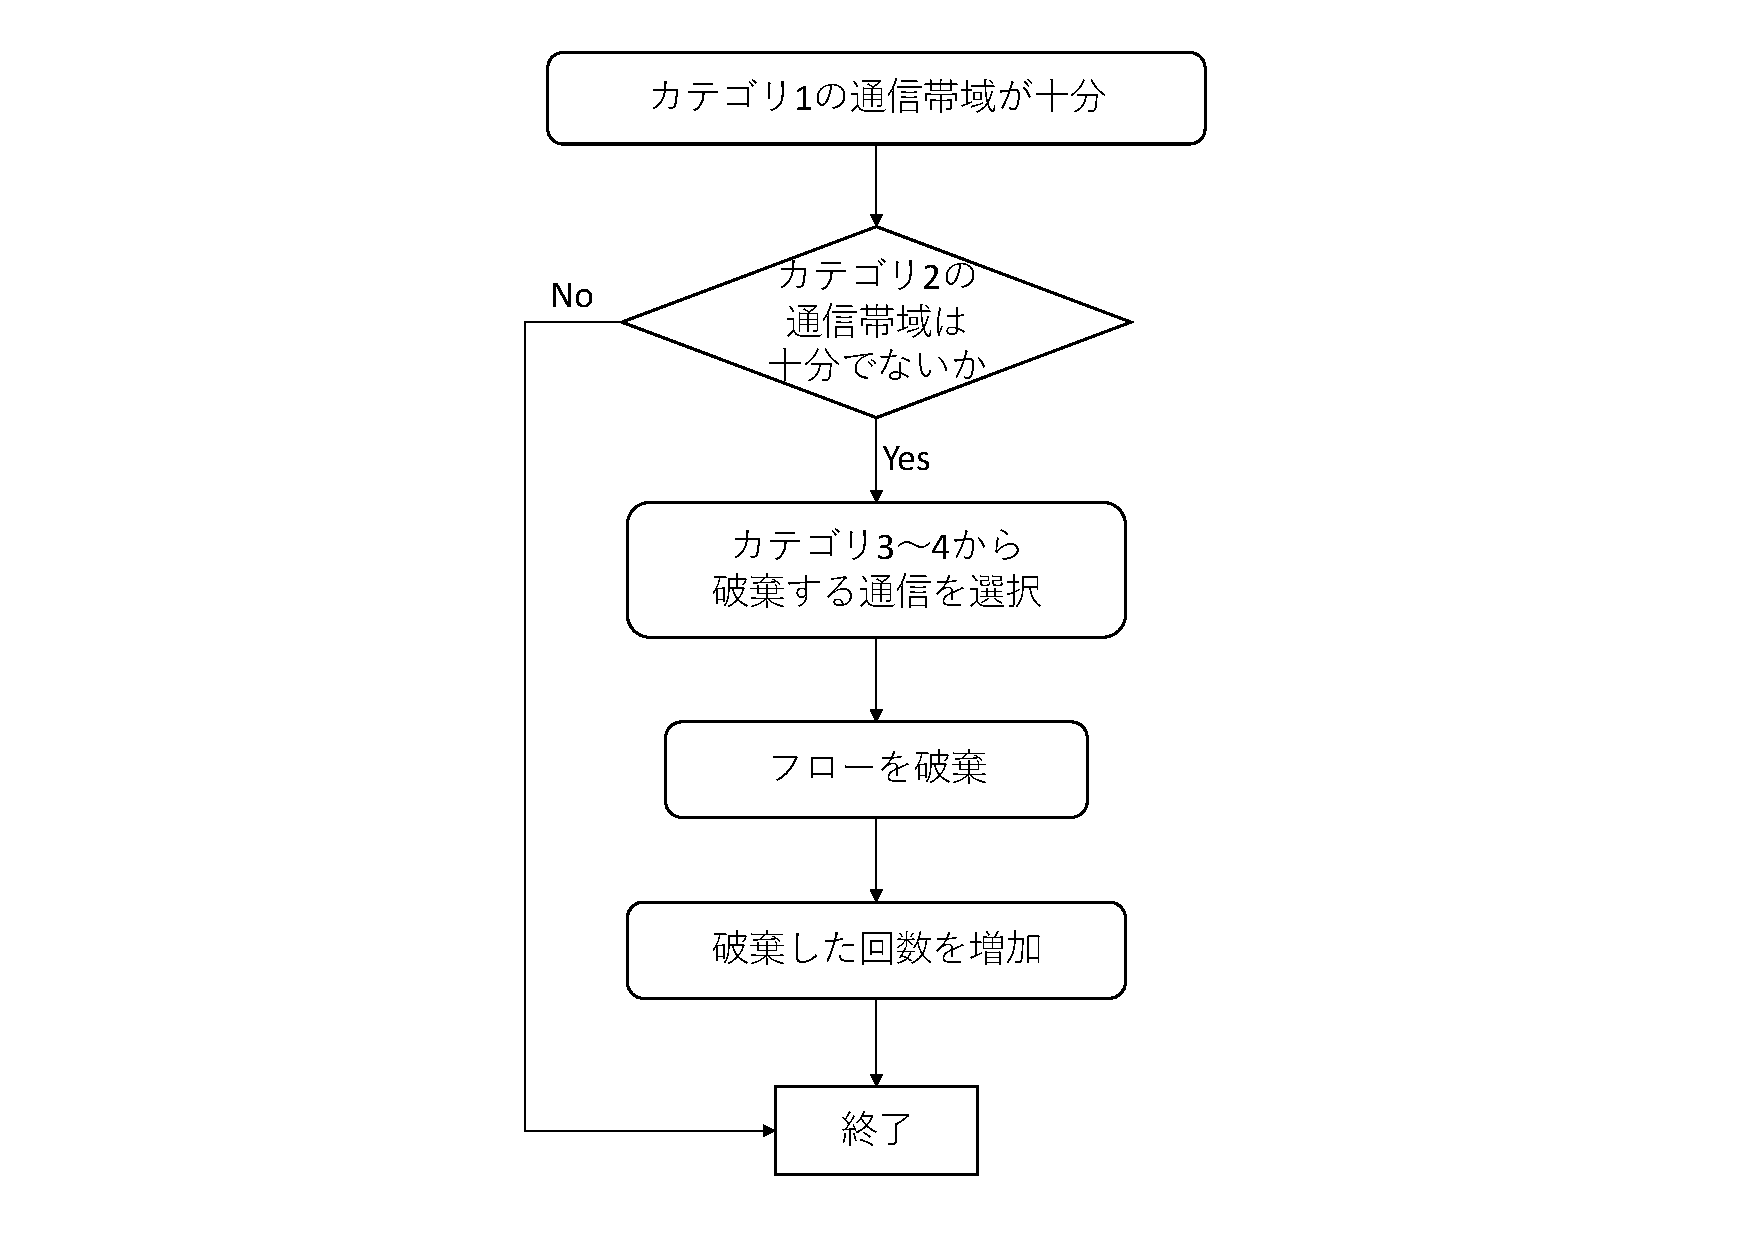
\includegraphics[width=\linewidth]{img/adomission_c2.pdf}
    \caption{カテゴリ2のためのアドミッション制御のフローチャート}
    \label{fig:adomission2}
  \end{figure}

  破棄するフローは基本的に優先度の低い通信のフローから選択する.
  しかし,ただ優先度の最も低いフローばかり選択していると,同じフローが破棄され続ける飢餓状態に陥る恐れがある.
  飢餓状態を防ぐため,各フローの破棄された回数を記録し,破棄するフローの選択に用いる.
  破棄するフローを選択する式を次に示す.\par

  \begin{equation}
    Min(w_2 dc_2, w_3 dc_3, w_4 dc_4)
  \end{equation}

  ここで,$w_2$,$w_3$,$w_4$は各カテゴリの通信に設定された重み,$dc_2$,$dc_3$,$dc_4$は各カテゴリの通信のフローが破棄された回数を表す.
  重みの大小関係は$w_2 > w_3 > w_4$であり,優先度の高い通信のフローほど破棄するフローに選択されづらい.
  フローが破棄された回数$dc$が増加するほど,そのフローが飢餓状態に近づいていることを意味するため,$dc$の増加に従い破棄するフローに選択されづらくなっている.\par
  $dc$を初期化せずに放置すると,$dc$の値は大きくなるが$dc_2$,$dc_3$,$dc_4$のそれぞれの差が小さくなるため,重み$w$の影響が小さくなってしまう.そのため,$dc$に閾値を設定し,$dc_2$,$dc_3$,$dc_4$のいずれかが閾値を超えた際に$dc$をリセットする.\par
  また,ホームネットワークのユーザや家庭の状況によっては,カテゴリ4の優先度の方がカテゴリ3の優先度より高くなる場合が発生する.
  例えば,火災が発生した場合,火災そのものを検知するカテゴリ1の通信に加えて,温度センサによって火の手がどこまで回っているかを把握することができるカテゴリ4の通信も重要であり,この時カテゴリ3よりもカテゴリ4の優先度の方が高く設定されるべきである.
  優先度の変更が必要になった場合,カテゴリ3に設定されていた$w_3$,$dc_3$とカテゴリ4に設定されていた$w_4$,$dc_4$の値を入れ替えることで,カテゴリ4の通信よりもカテゴリ3の通信が破棄するフローとして選択されやすくなる.

%\section{文献の引用の仕方}
%\label{sec:分権の引用の仕方}

%この文献\cite{LaTexWiki,渡辺豊2016}を参考にした.\par

%\section{図の挿入の仕方}
%\label{sec:図の挿入の仕方}

%図は以下のように挿入し,\figref{fig:sample1}と引用します.\par

%\begin{figure}[!tb]
%  \centering
%  
\includegraphics[width=\linewidth]{img/sample1.pdf}
%  \caption{サンプル画像1}
%  \label{fig:sample1}
%\end{figure}

%----------------------------------------------------------------------

\chapter{評価}
\label{chap:評価}

\section{評価環境}
\label{評価環境}

  提案手法の有効性を評価するにあたり,ネットワークエミュレータであるMininet\cite{Mininet}を用いてホームネットワークとISPサーバ間のネットワークを想定したネットワークを構築し,ネットワークシミュレーションを行った.
  構築したネットワークの構成を\figref{fig:experiment}に示す.\par

  \begin{figure}[!b]
    \centering
    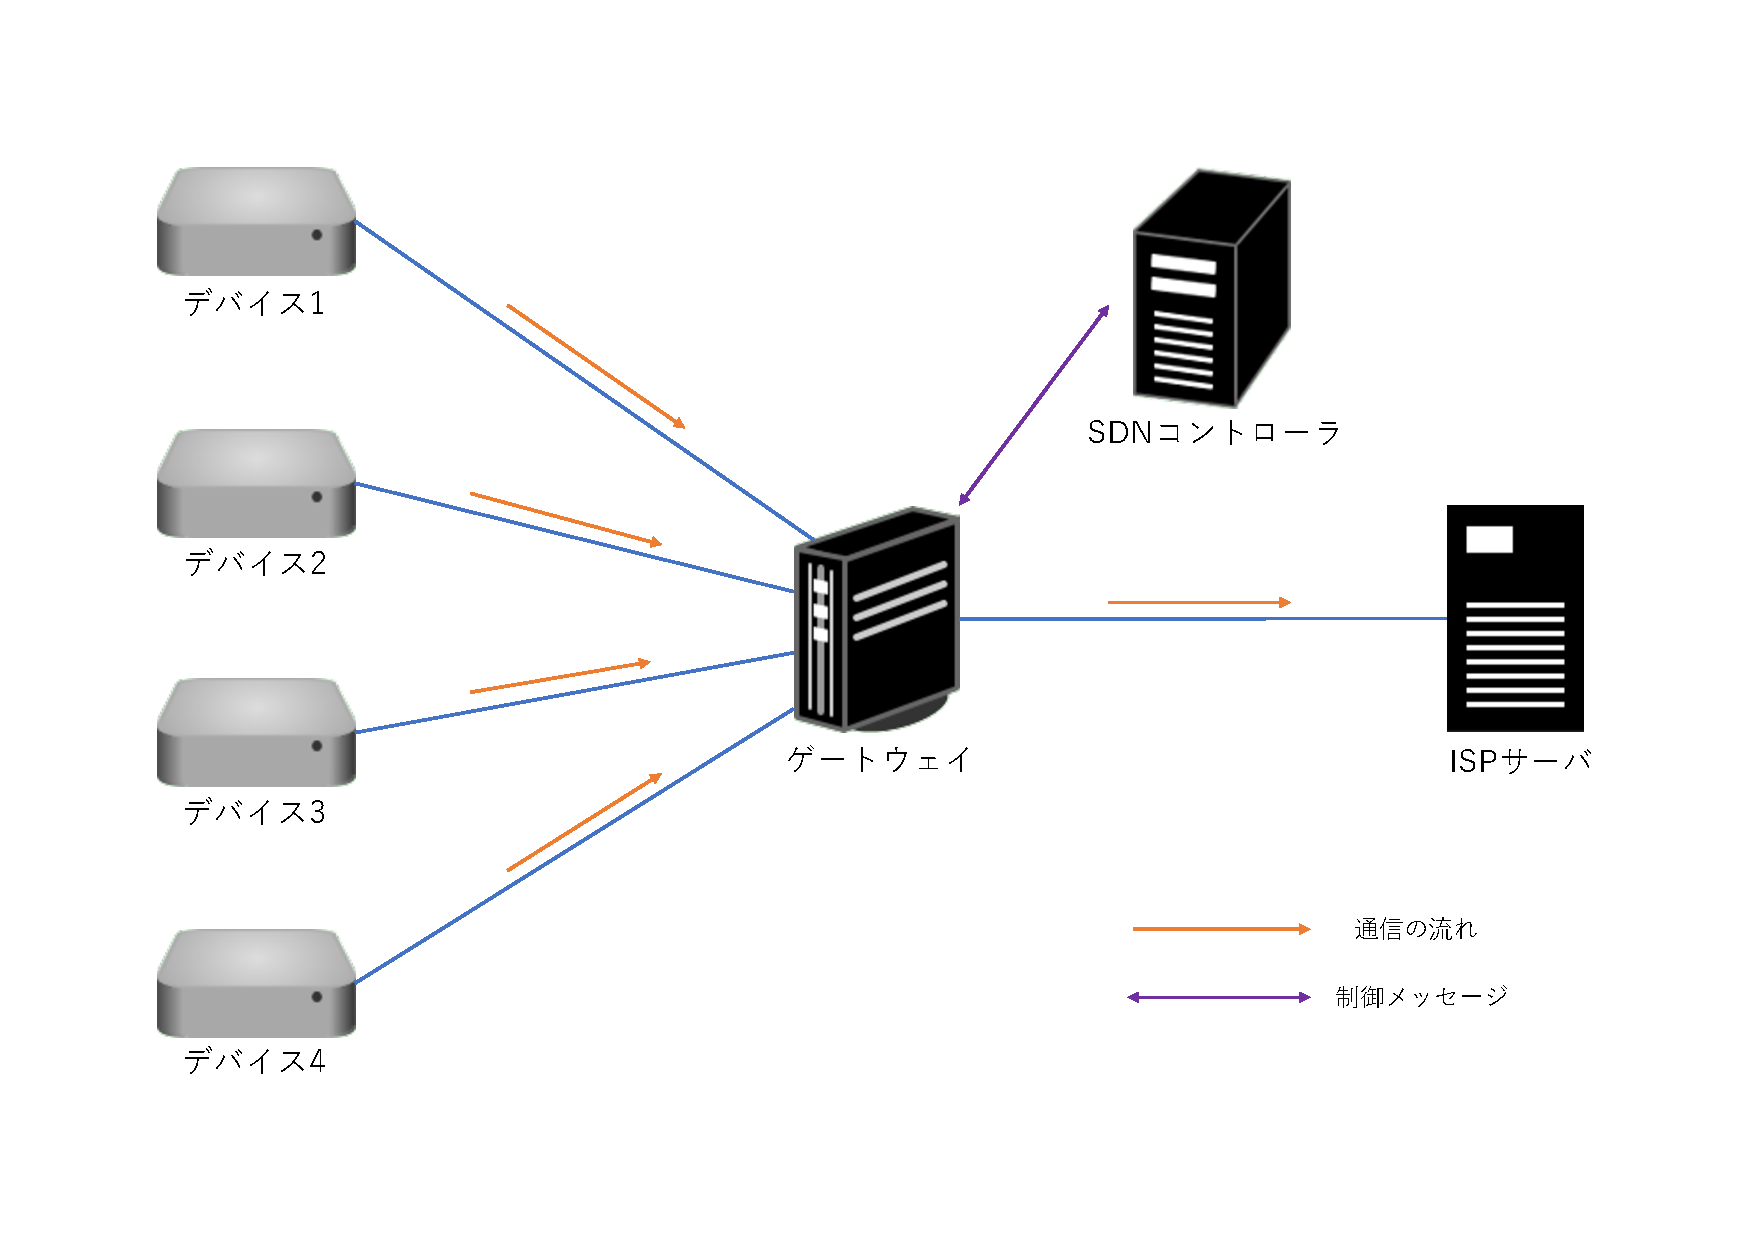
\includegraphics[width=\linewidth]{img/experiment.pdf}
    \caption{シミュレーションを行なったネットワーク構成}
    \label{fig:experiment}
  \end{figure}

  4つのデバイスおよびISPサーバはMininetのホスト,ゲートウェイはMininetのOpen VSwitchとして実装した.
  4つのデバイスはゲートウェイと接続しており,それぞれカテゴリ1\textasciitilde4の通信を行う.
  ゲートウェイはルータを経由せず,直接ISPサーバと接続している.
  通常,ホームネットワークとISPサーバ間の通信帯域はホームネットワーク内の通信帯域に比べて,デバイスまたはホームネットワークの数が少ない場合,提案する優先度制御にはルータの有無は影響しないため,上記のネットワーク構成によりシミュレーションを行なった.
  ゲートウェイはSDNコントローラと接続し,優先度制御に必要なメッセージをやり取りする.
  SDNコントローラには,SDN構築フレームワークであるRyu\cite{Ryu}を用いた.\par

  提案手法の有効性を評価するため,通信帯域が逼迫した際に優先度が高い通信の性能を測定する.
  通信帯域の逼迫を再現するため,各デバイスとゲートウェイ間のリンクおよびゲートウェイとISPサーバ間のリンクの通信帯域を1Mbpsに制限する.
  そして,TCP/IPパケットジェネレータおよびアナライザであるhping3\cite{hping3}を用いて,各デバイスからISPサーバへとパケットを送信する.パケット送信パラメータを\tabref{tab:packetParameter}に示す.

  \begin{table}[!tb]
    \caption{各デバイスのパケット送信パラメータ}
    \label{tab:packetParameter}
    \centering
    \begin{tabular}{cc}
      \hline
      送信間隔 & 1000ms\\
      データサイズ & 34464Byte\\
      パケット数 & 500\\
      \hline
    \end{tabular}
  \end{table}

  SDNコントローラは,各デバイスが接続されているゲートウェイの4つのポートが受信する通信量を監視し,15秒おきにアドミッション制御を行うか否かを決定する.
  各ポートごとに通信量の閾値を設定し,アドミッション制御の決定間隔の15秒間で各ポートが受信した総通信量が閾値を超えた場合,そのポートに接続されているデバイスの通信を行うのに十分な通信帯域がないと見なし,そのポートが行っている通信の優先度に応じてアドミッション制御が行われる.
  各ポートの閾値を\tabref{tab:threshold}に示す.
  SDNコントローラは\ref{sec:アドミッション制御}節に示した式を用いて破棄するフローを選択し,ゲートウェイにフローの破棄を指示する.
  指示を受けたゲートウェイは,そのフローを受信してもISPサーバへ送信せず破棄する.
  次に15秒経過して,アドミッション制御を行うか否かを判断する前に,破棄されていたフローを再度ゲートウェイに登録する.
  アドミッション制御の結果破棄するフローに再度選ばれた場合は,連続してフローが破棄される.
  別のフローが選択された場合は,先ほどまで破棄されていたフローの通信は再開され,新たに選択されたフローの通信が切断される.
  破棄するフローの選択には,\ref{sec:アドミッション制御}で述べた通り破棄された回数も優先度と同時に用いる.
  ここでは,各カテゴリの重みの初期値を$w_2=3$,$w_3=2$,$w_4=1$とした.\par

  \begin{table}[!tb]
    \caption{各ポートの通信量の閾値}
    \label{tab:threshold}
    \centering
    \begin{tabular}{cc}
      \hline
      カテゴリ1 & 100000Byte\\
      カテゴリ2 & 1000000Byte\\
      カテゴリ3 & 1000000Byte\\
      カテゴリ4 & 100000Byte\\
      \hline
    \end{tabular}
  \end{table}

  通信帯域が逼迫した際に優先度の高い通信の品質を改善できているかを評価するため,各優先度の通信のデバイスからISPサーバまでの実効スループット,デバイスがパケットを送信してからその応答がデバイスに返ってくるまでの遅延時間,送信するパケットの損失率を測定し,提案手法を用いない場合と比較する.
  また,優先度の動的な設定の有効性を評価するため,カテゴリ3とカテゴリ4の優先度が入れ替わった場合において,提案手法と固定された優先度分類を用いた優先度制御の実効スループット,遅延時間,パケットロス率を測定し比較する.
  さらに,リアルタイム性を考慮して分類したカテゴリ2とカテゴリ3について,破棄されたパケットのシーケンス番号を比較し,パケットの連続性からリアルタイム性について評価する.

\section{通信性能}
\label{sec:通信性能}

  提案手法を用いた場合と優先度制御を行わなかった場合との実効スループットの比較を\figref{fig:throughput_1}に示す.
  ここで,最も優先度が高い順に各通信を優先度1\textasciitilde4とし,それぞれカテゴリ1\textasciitilde4に対応する.
  提案手法を用いた場合の優先度1の実効スループットは228.84Mbps,優先度2の実効スループットは200.35Mbps,優先度3の実効スループットは143.37Mbps,優先度4の実効スループットは98.33Mbpsであった.
  一方,優先度制御を行わない場合の優先度1の実効スループットは163.59Mbps,優先度2の実効スループットは212.3Mbps,優先度3の実効スループットは216.89Mbps,優先度4の実効スループットは218.73Mbpsであった.

  \begin{figure}[!b]
    \centering
    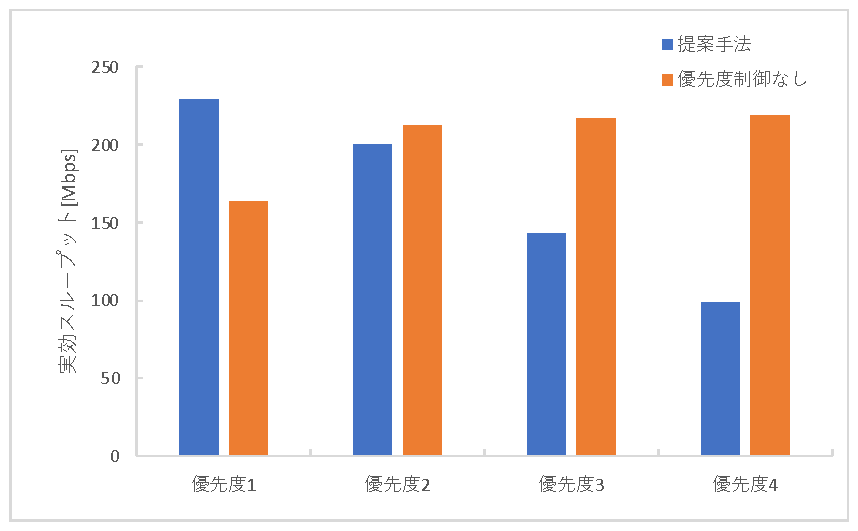
\includegraphics[width=\linewidth]{img/throughput_1.pdf}
    \caption{優先度制御しない場合との実効スループットの比較}
    \label{fig:throughput_1}
  \end{figure}

  提案手法を用いた場合と優先度制御を行わなかった場合との遅延時間の比較を\figref{fig:RTT_1}に示す.
  提案手法を用いた場合の優先度1の平均遅延時間は8634.0ms,優先度2の平均遅延時間は8601.9ms,優先度3の平均遅延時間は8342.6ms,優先度4の平均遅延時間は8536.4msであった.
  また,優先度制御を行わない場合の優先度1の平均遅延時間は9026.7ms,優先度2の平均遅延時間は9392.9ms,優先度3の平均遅延時間は9256.6ms,優先度4の平均遅延時間は9486.7msであった.

  \begin{figure}[!b]
    \centering
    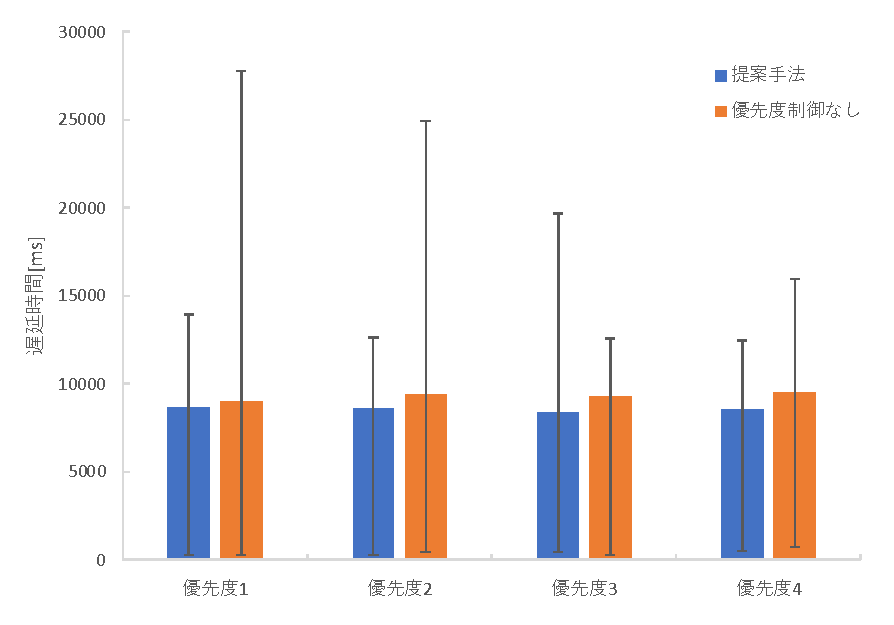
\includegraphics[width=\linewidth]{img/RTT_1.pdf}
    \caption{優先度制御しない場合との遅延時間の比較}
    \label{fig:RTT_1}
  \end{figure}

  提案手法を用いた場合と優先度制御を行わなかった場合とのパケット損失率の比較を\figref{fig:packetloss_1}に示す.
  提案手法を用いた場合の優先度1のパケット損失率は17\%,優先度2の平均遅延時間は28\%,優先度3の平均遅延時間は48\%,優先度4のパケット損失率は65\%であった.
  一方,提案手法を用いた場合の優先度1のパケット損失率は41\%,優先度2の平均遅延時間は23\%,優先度3の平均遅延時間は22\%,優先度4のパケット損失率は21\%であった.

  \begin{figure}[!b]
    \centering
    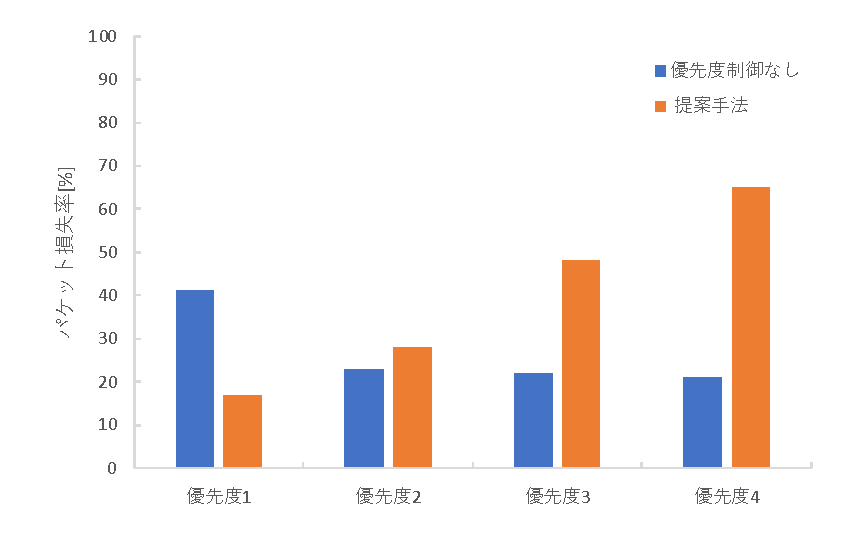
\includegraphics[width=\linewidth]{img/packetloss_1.pdf}
    \caption{優先度制御しない場合とのパケット損失率の比較}
    \label{fig:packetloss_1}
  \end{figure}

\section{動的な優先度分類}
\label{sec:動的な優先度分類}

  カテゴリ3とカテゴリ4の優先度が入れ替わった場合,すなわちカテゴリ1=優先度1,カテゴリ2=優先度2,カテゴリ4=優先度3,カテゴリ3=優先度4の場合について,提案手法を用いて動的に優先度分類を行なった通信性能「と固定された優先度分類を用いた通信性能を比較する.
  提案手法を用いた場合と固定された優先度分類を用いた場合との実効スループットの比較を\figref{fig:throughput_2}に示す.
  提案手法を用いた場合の優先度1の実効スループットは246.98Mbps,優先度2の実効スループットは204.03Mbps,優先度3の実効スループットは182.89Mbps,優先度4の実効スループットは99.26Mbpsであった.
  一方,優先度制御を行わない場合の優先度1の実効スループットは240.79Mbps,優先度2の実効スループットは194.84Mbps,優先度3の実効スループットは103.85Mbps,優先度4の実効スループットは172.78Mbpsであった.

  \begin{figure}[!b]
    \centering
    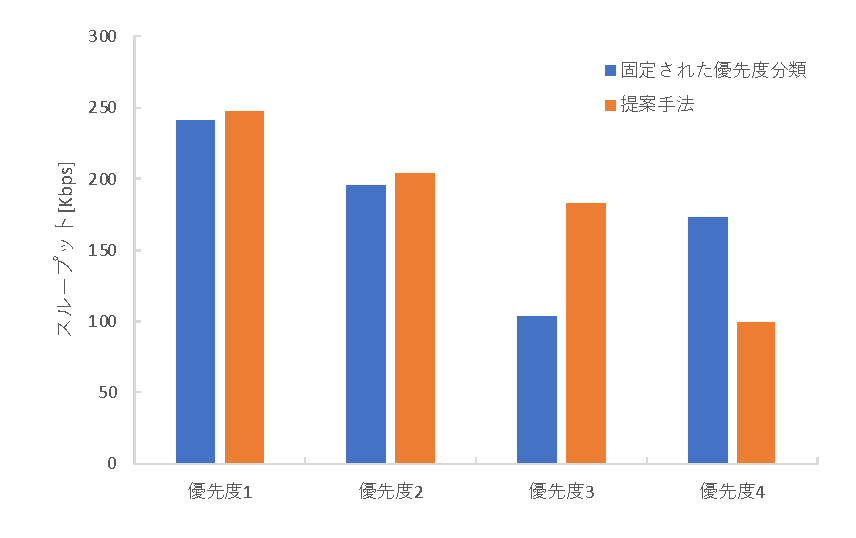
\includegraphics[width=\linewidth]{img/throughput_2.pdf}
    \caption{固定された優先度分類との実効スループットの比較}
    \label{fig:throughput_2}
  \end{figure}

  提案手法を用いた場合と優先度制御を行わなかった場合との遅延時間の比較を\figref{fig:RTT_2}に示す.
  提案手法を用いた場合の優先度1の平均遅延時間は6704.9ms,優先度2の平均遅延時間は6532.8ms,優先度3の平均遅延時間は6816.8ms,優先度4の平均遅延時間は6561.3msであった.
  また,優先度制御を行わない場合の優先度1の平均遅延時間は6802.5ms,優先度2の平均遅延時間は6834.7ms,優先度3の平均遅延時間は6276.8ms,優先度4の平均遅延時間は6745.1msであった.

  \begin{figure}[!b]
    \centering
    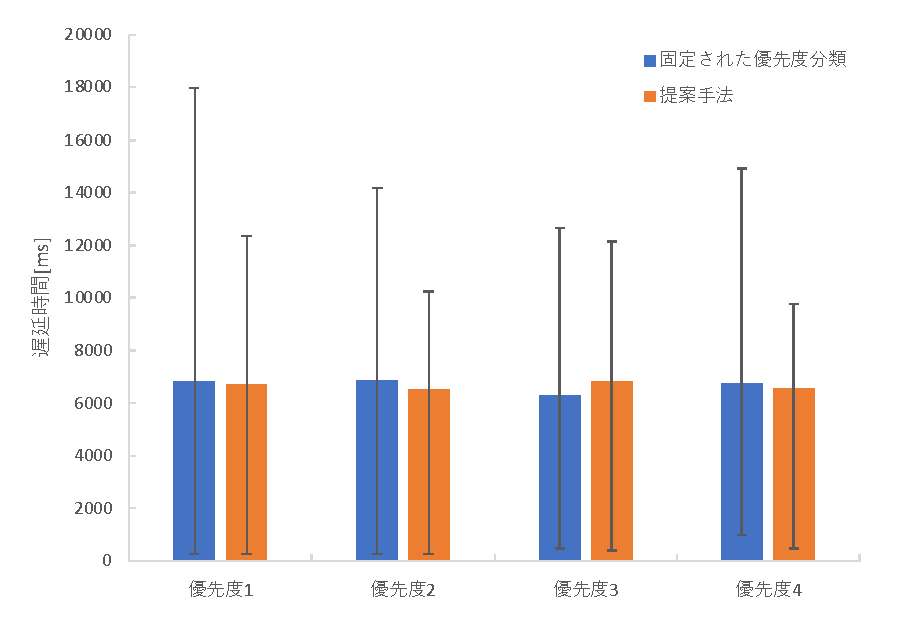
\includegraphics[width=\linewidth]{img/RTT_2.pdf}
    \caption{固定された優先度分類との遅延時間の比較}
    \label{fig:RTT_2}
  \end{figure}

  提案手法を用いた場合と優先度制御を行わなかった場合とのパケット損失率の比較を\figref{fig:packetloss_2}に示す.
  提案手法を用いた場合の優先度1のパケット損失率は10\%,優先度2の平均遅延時間は26\%,優先度3の平均遅延時間は34\%,優先度4のパケット損失率は64\%であった.
  一方,提案手法を用いた場合の優先度1のパケット損失率は13\%,優先度2の平均遅延時間は30\%,優先度3の平均遅延時間は63\%,優先度4のパケット損失率は38\%であった.

  \begin{figure}[!b]
    \centering
    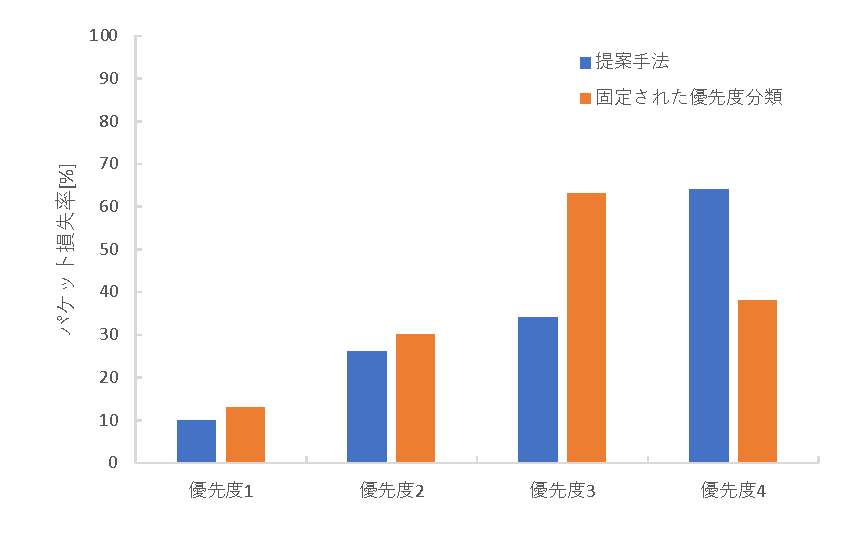
\includegraphics[width=\linewidth]{img/packetloss_2.pdf}
    \caption{固定された優先度分類とのパケット損失率の比較}
    \label{fig:packetloss_2}
  \end{figure}

\section{通信のリアルタイム性}
\label{sec:通信のリアルタイム性}

  \ref{sec:通信の分類}節で,リアルタイム性の点から音声・映像データの通信をカテゴリ2とカテゴリ3に分類した.
  カテゴリ2とカテゴリ3のそれぞれの破棄されたパケットのシーケンス番号を比較することで,パケットの連続性からリアルタイム性を評価する.
  それぞれのパケットが到達/破棄されたシーケンス番号を\figref{fig:realtime}に示す.
  パケット到達の値が1の時はパケットが正常に到達しており,0の時はパケットが破棄されていることを表す.
  カテゴリ2では1回の連続した破棄を含む6回の破棄があったのに対して,カテゴリ3では1回の連続した破棄を含む7回の破棄があった.

  \begin{figure}[!b]
    \centering
    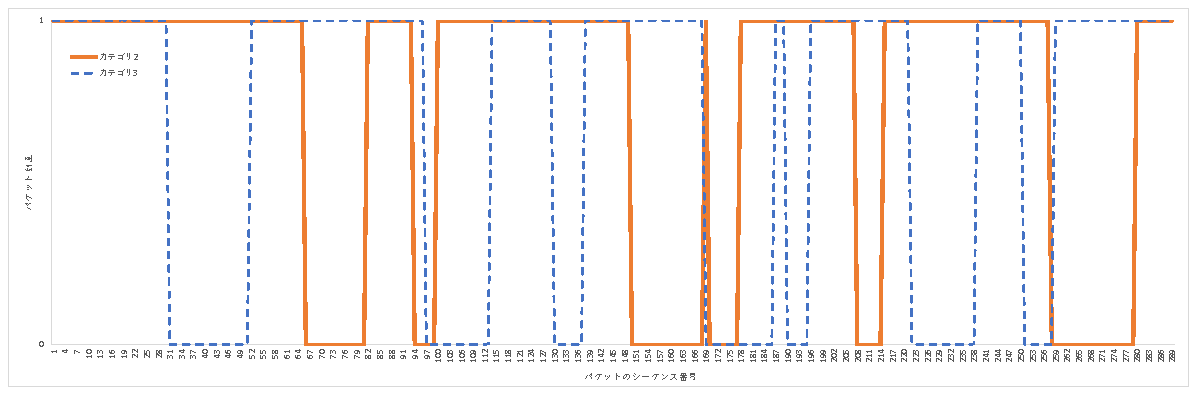
\includegraphics[width=\linewidth]{img/realtime.pdf}
    \caption{パケットの到達/破棄}
    \label{fig:realtime}
  \end{figure}

%----------------------------------------------------------------------

\chapter{考察}
\label{chap:考察}

  ここでは,\ref{chap:評価}章で述べた結果をもとに提案手法を考察する.
  \ref{sec:通信性能}節の結果をもとに,優先度制御の有効性を考察する.
  次に,\ref{sec:動的な優先度分類}節の結果から,動的な優先度分類の有効性を考察する.
  また,\ref{sec:通信のリアルタイム性}節の結果をもとに,カテゴリ2とカテゴリ3のリアルタイム性を比較し分析する.\par

  \figref{fig:throughput_1}に示すように,最も優先度の高い優先度1の通信のスループットは,提案手法を用いた場合の方が優先度制御しない場合と比較して向上している.
  しかし,優先度2\textasciitilde4の通信ではスループットが低下しており,通信全体のスループットは低下している.
  また,\figref{fig:packetloss_1}に示すように,優先度1の通信のパケット損失率は改善してるが,優先度2\textasciitilde4の通信のパケット損失率は増加した.
  これは,提案手法では各ポートに設定した通信量の閾値を超えた際にアドミッション制御を行うため,まだ通信帯域が逼迫しきっておらず,パケットを送信する余裕があったがパケットを破棄してしまったことが原因と考察される.
  一方,優先度制御を用いない場合は,通信帯域の限界のみでしかパケットの損失が発生しないため,提案手法を用いた場合と比較して通信全体の実効スループットとパケット損失率は高い品質を示した.
  アドミッション制御を,通信量の閾値をもとに行うのではなく,通信帯域の逼迫率をもとに行うことで,実効スループットとパケット損失率の改善が可能である.\par

  \figref{fig:RTT_1}に示すように,デバイスがパケットを送信してからその応答がデバイスに返ってくるまでの遅延時間は,提案手法を用いた場合が優先度制御しない場合と比較して軽減した.
  これは,優先度制御を用いない場合では,通信帯域が逼迫した際にTCPの確認応答と再送制御が行われるため遅延時間が増加するのに対して,提案手法では通信量が閾値を超えた場合にパケットが破棄されるため,確認応答と再送制御がそもそも行われず,その分遅延時間が軽減されていると考察される.
  通信帯域の逼迫率を監視し,パケットの到達が見込めない時はパケットを破棄することで,遅延時間を軽減することが可能である.\par

  次に,提案手法の動的な優先度分類について考察する.
  \figref{fig:throughput_2}に示すように,提案手法を用いた場合では優先度の変更に合わせてアドミッション制御を行なったため,カテゴリ4=優先度3の実効スループットがカテゴリ3=優先度4の実効スループットよりも高くなっている.
  一方,固定された優先度分類では,カテゴリ4=優先度3の実効スループットがカテゴリ3=優先度4の実効スループットよりも低くなっており,優先度の変化に対応できていない.
  また,パケット損失率についても,提案手法ではカテゴリ4=優先度3のパケット損失率がカテゴリ3=優先度4のパケット損失率よりも低下しているのに対して,固定した優先度分類ではカテゴリ4=優先度3のパケット損失率がカテゴリ3=優先度4のパケット損失率より高くなっている.
  動的な優先度分類によって,優先度の変更に対応した優先度制御を実現した.\par

  しかし,遅延時間については,\figref{fig:RTT_2}からわかるように,提案手法を用いた場合,固定された優先度分類を用いた場合ともに,カテゴリ4=優先度3とカテゴリ3=優先度4で動的な優先度分類が有効に作用した結果は見られない.
  提案手法を用いた場合の遅延時間は固定された優先度分類を用いた場合の遅延時間と比較して最大遅延時間や平均遅延時間が軽減されているが,どちらも\figref{fig:RTT_1}の提案手法を用いた場合の遅延時間より小さいことから,誤差の範囲内であると考察される.
  上で考察したようにパケットの破棄が遅延時間の軽減に繋がるため,実際のホームネットワークで長時間の動的な優先度制御では遅延時間の軽減が可能である.\par

  最後に通信のリアルタイム性について考察する.
  \figref{fig:realtime}に示すように,リアルタイム性の高い音声・映像データの通信であるカテゴリ2ではリアルタイム性の低い音声・映像データの通信であるカテゴリ3と比較して,パケットが破棄された回数が1回少なく,パケット到達が1の値を連続してとる時間も長いことから,提案手法ではカテゴリ2のリアルタイム性を向上できている.
  \ref{sec:アドミッション制御}の式に示した$w_2$の値を調整することで,通信帯域やホームネットワークの状況に応じたリアルタイム性の向上が可能である.

%----------------------------------------------------------------------
% おわりに
%----------------------------------------------------------------------
\chapter{おわりに}
\label{chap:おわりに}

%まとめを書きましょう.800字から1000字ぐらいでまとめてください.背景,解決すべき問題点,提案内容,結果,考察,研究の意義などを含めて記載してください.結果については,過去形(・・・実施した.・・・評価した.・・・確認した.など)で記載してください.

  ホームネットワークの拡張や複雑化に伴い,SDNのホームネットワークへの適用が期待されている.
  ホームネットワークにはデータ特性が異なる通信が混在するため,データ特性から通信の優先度を分類し,通信帯域に応じて優先度制御を行う必要がある.
  また,ホームネットワークはユーザや時間帯による通信の種類と量の変動が大きく,ユーザや家庭の状況によって通信の重要度や需要も変化するため,優先度分類を動的に行う必要がある.
  これまで提案された優先度分類ではリアルタイム性が考慮されておらず,通信帯域の逼迫や優先度制御に伴うパケットロスの通信への影響が大きかった.
  また,固定された優先度分類を用いていたため,優先度に変更が求められる状況に対応した優先度制御ができなかった.\par
  本論文では,重要度やQoS要件,リアルタイム性といったデータ特性から通信を4つのカテゴリに分類した.
  また,通信帯域が逼迫した際に,通信の優先度に対応した重みとこれまで破棄された回数から新たに破棄するアドミッション制御を提案した.
  さらに,優先度の変更が必要な際には,通信の優先度に対応した重みとこれまで破棄された回数をカテゴリ間で入れ替えることで,動的な優先度分類を提案した.\par
  ホームネットワークを想定したネットワークを構築し,ネットワークシミュレーションを行うことで提案手法の有効性を検証した.
  優先度制御を行わない場合と比較して,優先度の高い通信の実効スループットとパケット損失率を改善した.
  また,固定された優先度分類と比較して,優先度に変更があった場合でも,動的に優先度分類を行い優先度に応じた優先度制御を実現した.
  さらに,リアルタイム性を考慮して分類した通信について,パケットの破棄された回数や連続して到達した時間からリアルタイム性の向上を示した.

%----------------------------------------------------------------------
% 謝辞
%----------------------------------------------------------------------
% サンプル
% 本研究を進めるにあたって,多大なご指導とご支援を賜りました同志社大学理工学部の佐藤健哉教授に心より感謝致します.また,3年間研究生活を共に過ごし,研究に就職活動と共に乗り越えたネットワーク情報システム研究室の同期,研究・就職活動の相談に乗ってくださった先輩,研究室生活で慕ってくれた後輩,さらに様々な場面で支えてくれた家族と友人へ感謝します.
%----------------------------------------------------------------------
\chapter*{謝辞}
\addcontentsline{toc}{chapter}{謝辞}  % 章番号のない章を目次に表示させる
\label{sec:Acknowledgments}

%謝辞には章番号をつけなくてもよいので,\verb|\chapter*{}| という具合に書きます.

  本研究を進めるにあたって,多大なご指導とご支援を賜りました同志社大学理工学部の佐藤健哉教授に心より感謝いたします.
  また,研究内容について親身にアドバイスをくださった山本浩太郎先輩をはじめとしたネットワーク情報システム研究室のみなさまには,大変お世話になりました.
  さらに,学校生活や研究活動を支えて支えてくれた友人と家族へ感謝いたします.

%----------------------------------------------------------------------
% 付録
%----------------------------------------------------------------------
%\appendix
%\chapter{ソースコード}
%\label{apndx:src}

%プログラム文とかを書きたい場合は,以下のようにしてみます.\verb|\usepackage{ascmac}|して\verb|screen| 環境を使うと,枠がつきます.

%\begin{screen}\begin{verbatim}
%#include <iostream>
%using namespace std;

%int main() {
%  for(int i = 1; i <= 5; i++) {
%    cout << "こんにちは, C++ の世界! " << i << endl;
%  }
%  return 0;
%}
%\end{verbatim}\end{screen}

%----------------------------------------------------------------------
% 参考文献
%----------------------------------------------------------------------
\renewcommand{\bibname}{参考文献}

% thebibliography を利用する場合は以下を使用(拘りがなければこちらでOK)
\begin{thebibliography}{99}
  \bibitem{NEC} NEC, \url{https://jpn.nec.com/sdn/about_sdn.html}(参照:2022/1).
  \bibitem{ガイドライン} 総務省,帯域制御の運用基準に関するガイドライン(改定). 2019.
  \bibitem{Framework} Hung-Chin Jang,Chi-Wei Huang and Fu-Ku Yeh,Design
  A Bandwidth Allocation Framework for SDN Based Smart
  Home,\textit{2016 IEEE 7th Annual Information Technology,
  Electronics and Mobile Communication Conference (IEMCON)},
  pp.1-6,2016.
  \bibitem{Framework2} Hung-Chin Jang and Jian-Ting Lin,SDN Based QoS Aware Bandwidth Management Framework of ISP for Smart Homes,\textit{2017 IEEE SmartWorld, Ubiquitous Intelligence \& Computing, Advanced \& Trusted Computed, Scalable Computing \& Communications, Cloud \& Big Data Computing, Internet of People and Smart City Innovation (SmartWorld/SCALCOM/UIC/ATC/CBDCom/IOP/SCI)},pp.1-7,2017.
  \bibitem{AQRA} Guo-Cin Deng and Kuochen Wang,An Application-aware QoS Routing Algorithm for SDN-based IoT Networking,\textit{2018 IEEE Symposium on Computers and Communications (ISCC)}, pp.186-191,2018.
  \bibitem{Mininet} Mininet.
  \bibitem{Ryu} Ryu.
  \bibitem{hping3} hping3.
\end{thebibliography}

% BibTex を利用する場合は以下を使用(初めての人には難しいかも)
% \bibliographystyle{junsrt}
% \bibliography{myref}

% 以下は上記どちらを利用する場合も必要
\label{chap:Bibiliography}
\addcontentsline{toc}{chapter}{参考文献}  % 章番号のない章を目次に表示させる

%----------------------------------------------------------------------
% 研究業績
%----------------------------------------------------------------------
\renewcommand{\bibname}{研究業績}

\begin{thebibliography}{99}
  \bibitem{} 国本 典晟,細野 航平,滕 睿,佐藤 健哉,"ホームネットワークにおけるデータ特性を考慮したSDNによる優先度制御手法," 情報処理学会 第84回全国大会.2022.(発表予定)
\end{thebibliography}

\label{chap:Publications}
\addcontentsline{toc}{chapter}{研究業績}

%----------------------------------------------------------------------
\end{document}
%----------------------------------------------------------------------
